\chapter{Experiments}
\label{ch:experiments}
\section{NAO}
Brief description of NAO v5 (which is running BHuman).

\section{Simple Staircase}
Staircase from 1cm to 5cm. Limitations of the robot.
\begin{figure}
  \centering
  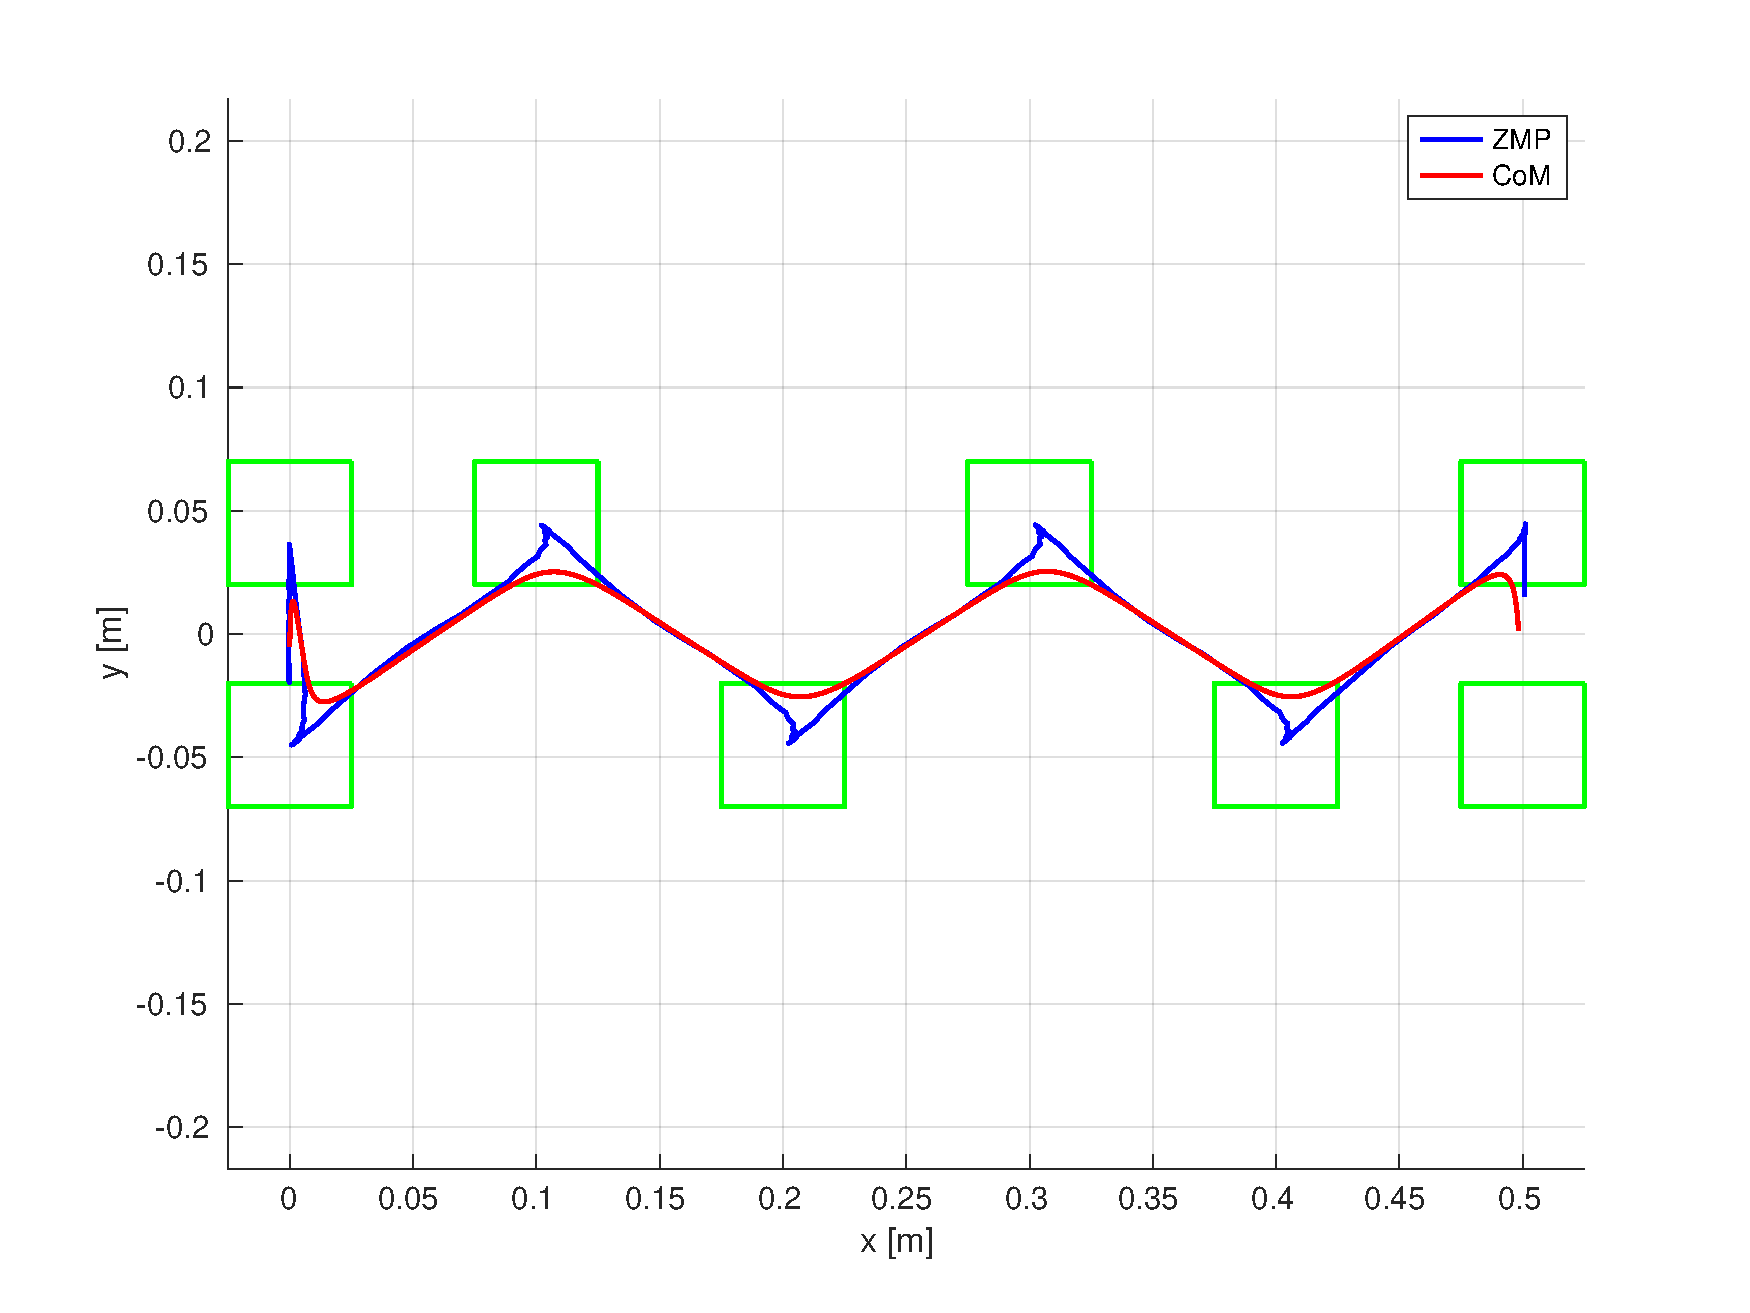
\includegraphics[width=\textwidth]
      {figures/experiments/simple-staircase/xy-plot-4cm.pdf}
  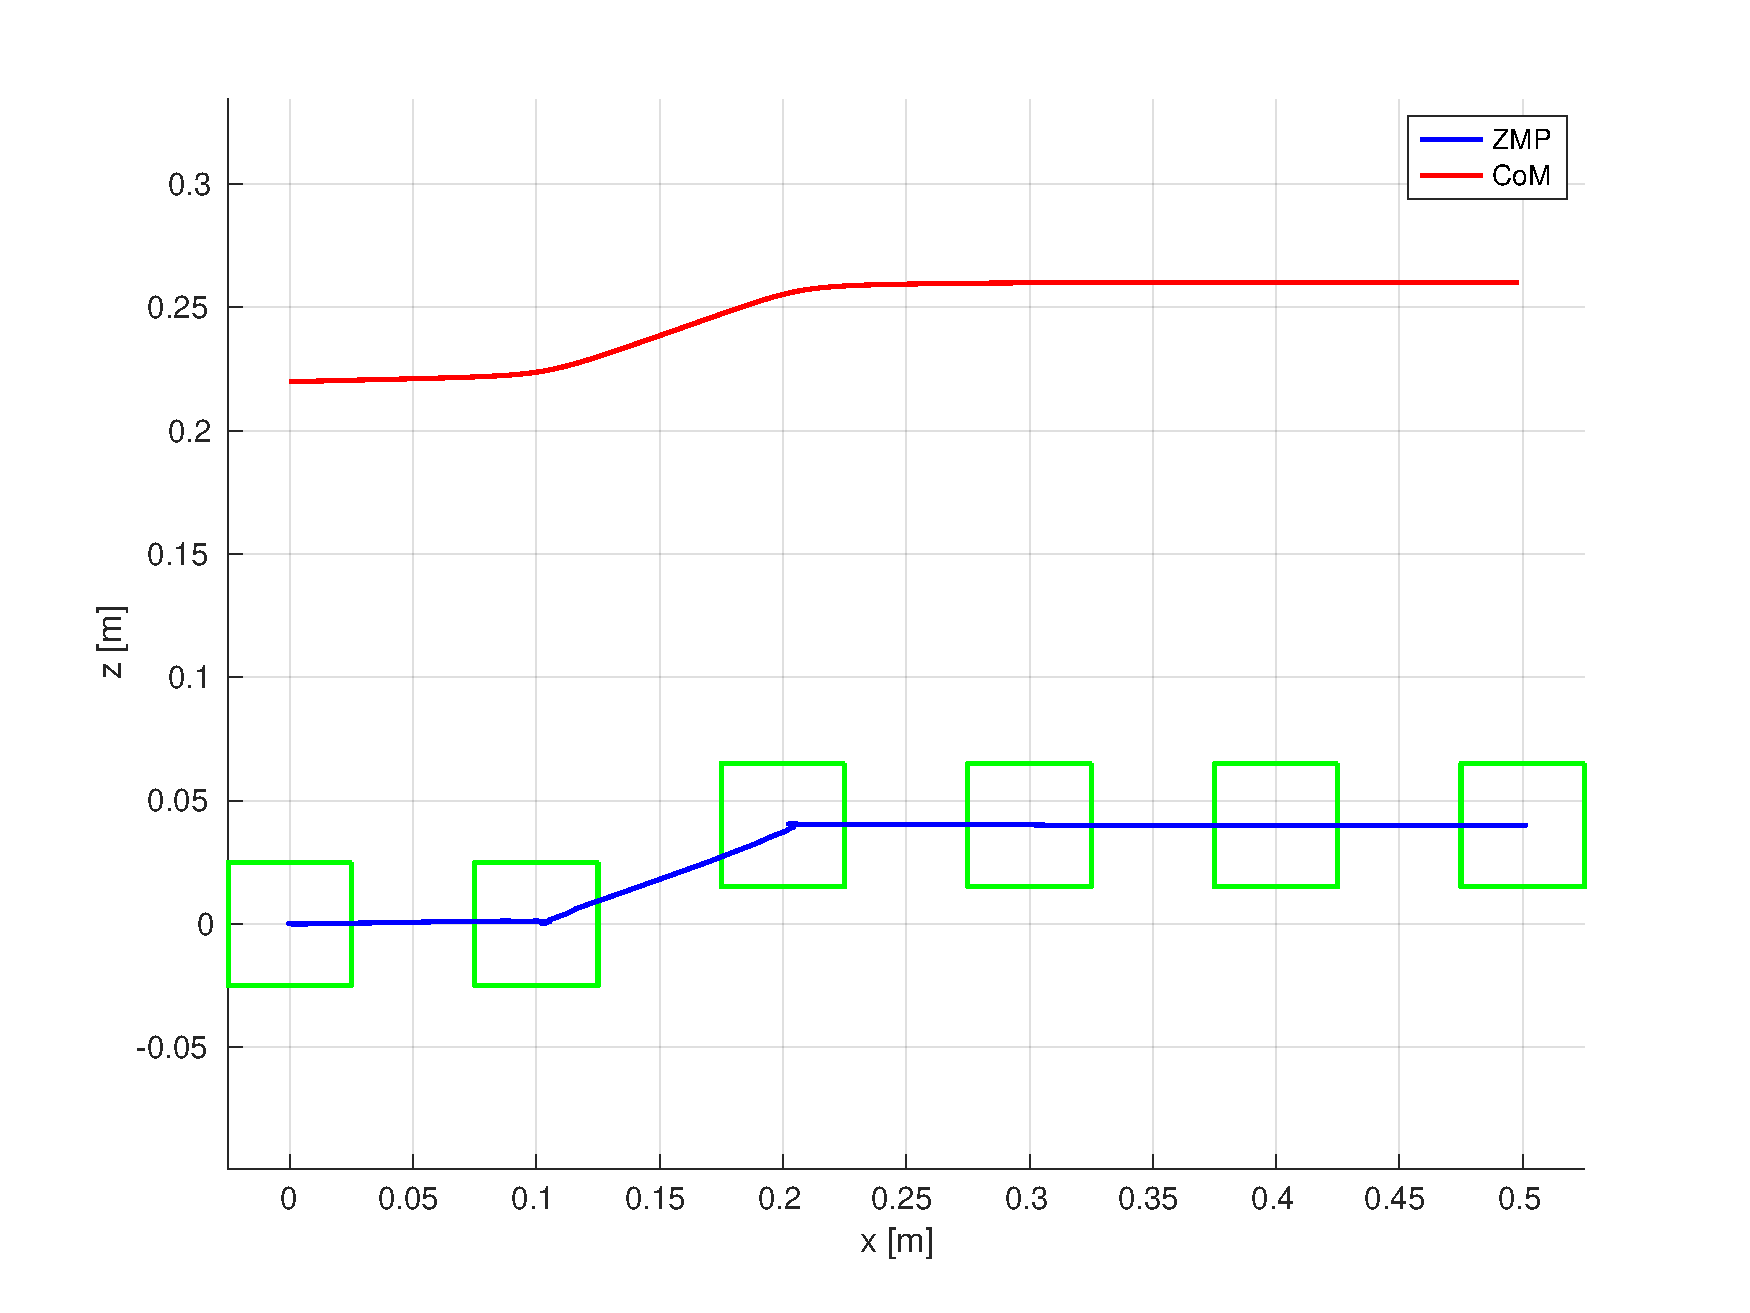
\includegraphics[width=\textwidth]
      {figures/experiments/simple-staircase/xz-plot-4cm.pdf}
  \caption{The plots show how the CoM and the ZMP vary with respect to the
		footsteps in the scenario ``Simple Staircase''.
    The green boxes represent the footsteps.}
  \label{fig:experiments:simple-staircase:comzmp}
\end{figure}

\section{Multiple Staircases}
Two consecutive staircases of 2cm.

\subsection{Upstairs}
Upstairs.
\begin{figure}
  \begin{subfigure}{0.48\textwidth}
    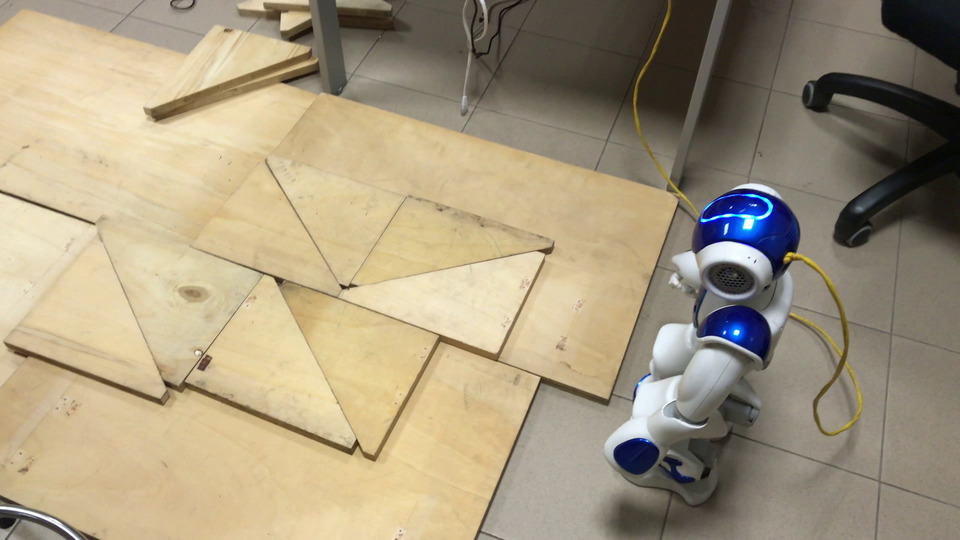
\includegraphics[width=\linewidth]
      {figures/experiments/multiple-staircases/upstairs/video/01.png}
    \caption{Starting position}
    \label{fig:exp:ms:up:frame1}
  \end{subfigure}\hspace*{\fill}
  \begin{subfigure}{0.48\textwidth}
    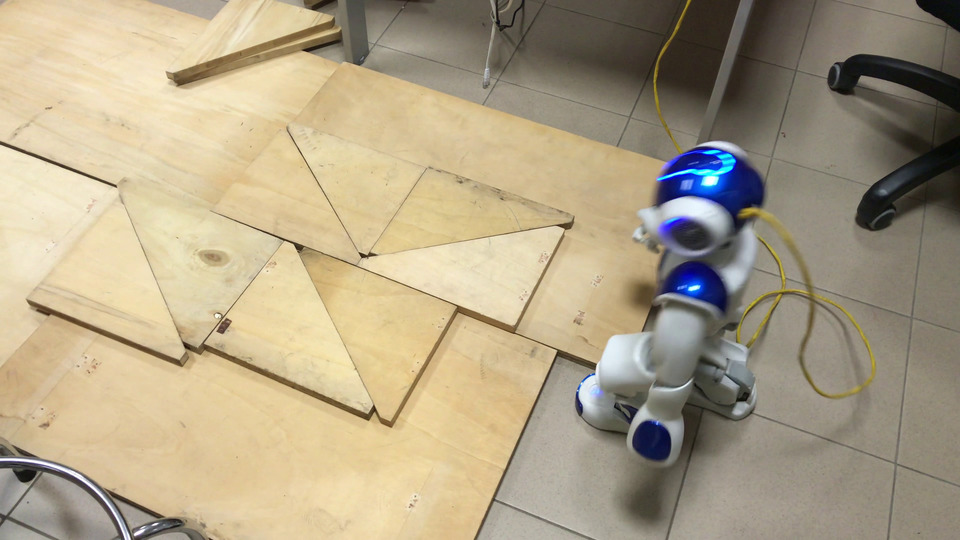
\includegraphics[width=\linewidth]
      {figures/experiments/multiple-staircases/upstairs/video/02.png}
    \caption{First step}
  \end{subfigure}
  \begin{subfigure}{0.48\textwidth}
    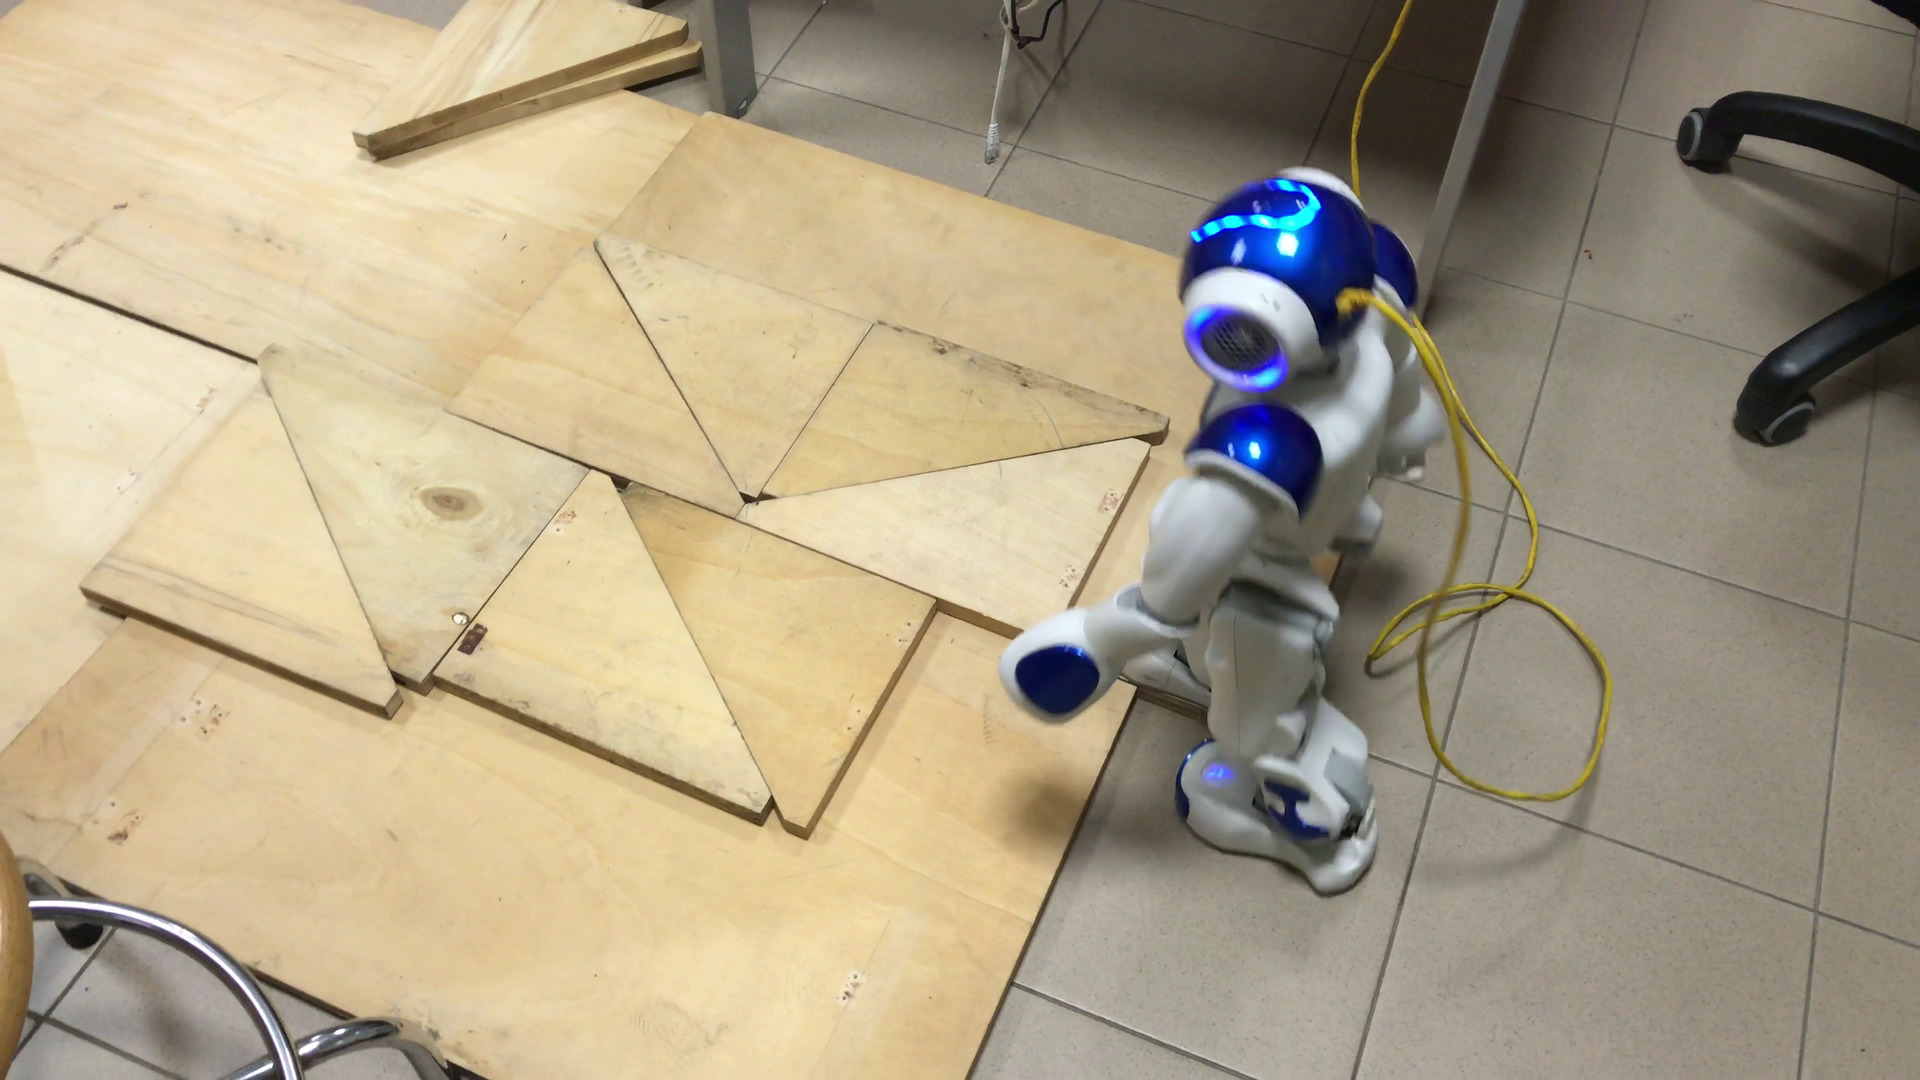
\includegraphics[width=\linewidth]
      {figures/experiments/multiple-staircases/upstairs/video/03.png}
    \caption{Second step}
  \end{subfigure}\hspace*{\fill}
  \begin{subfigure}{0.48\textwidth}
    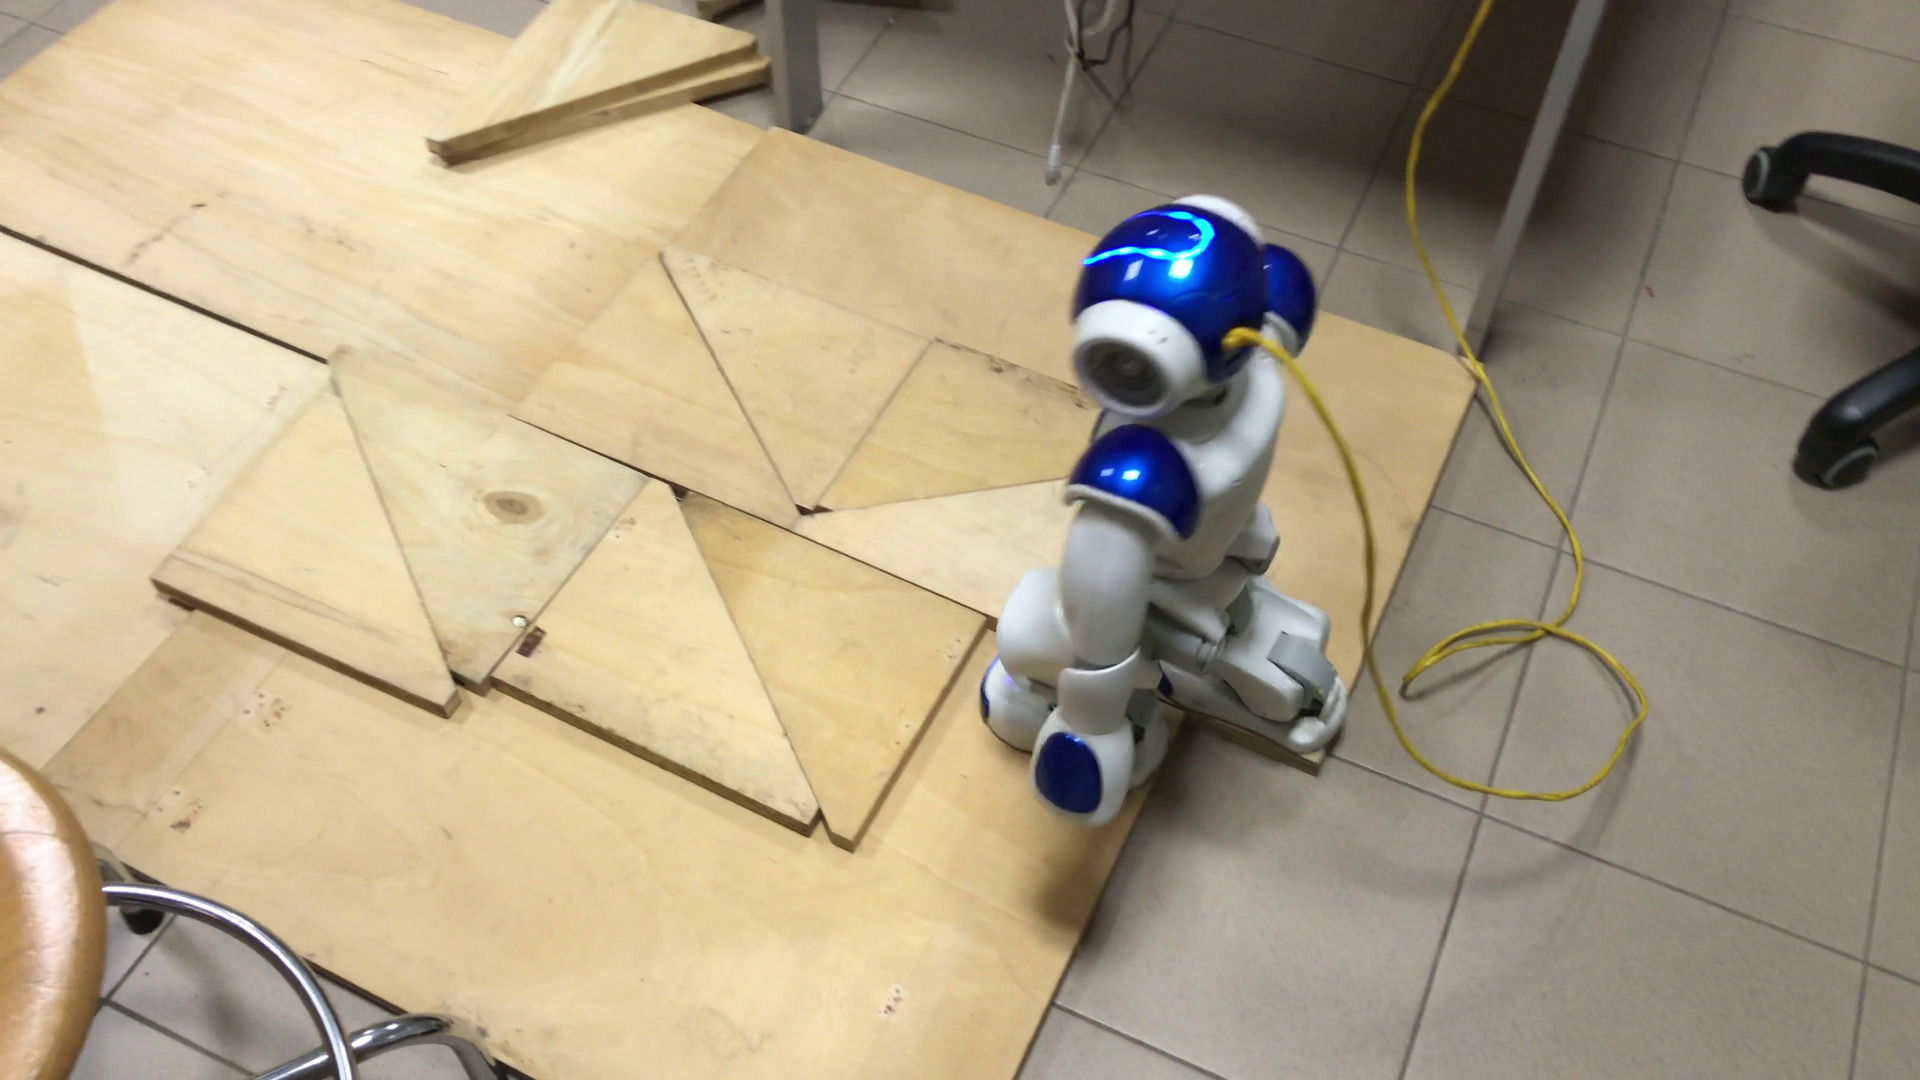
\includegraphics[width=\linewidth]
      {figures/experiments/multiple-staircases/upstairs/video/04.png}
    \caption{Third step}
  \end{subfigure}
  \begin{subfigure}{0.48\textwidth}
    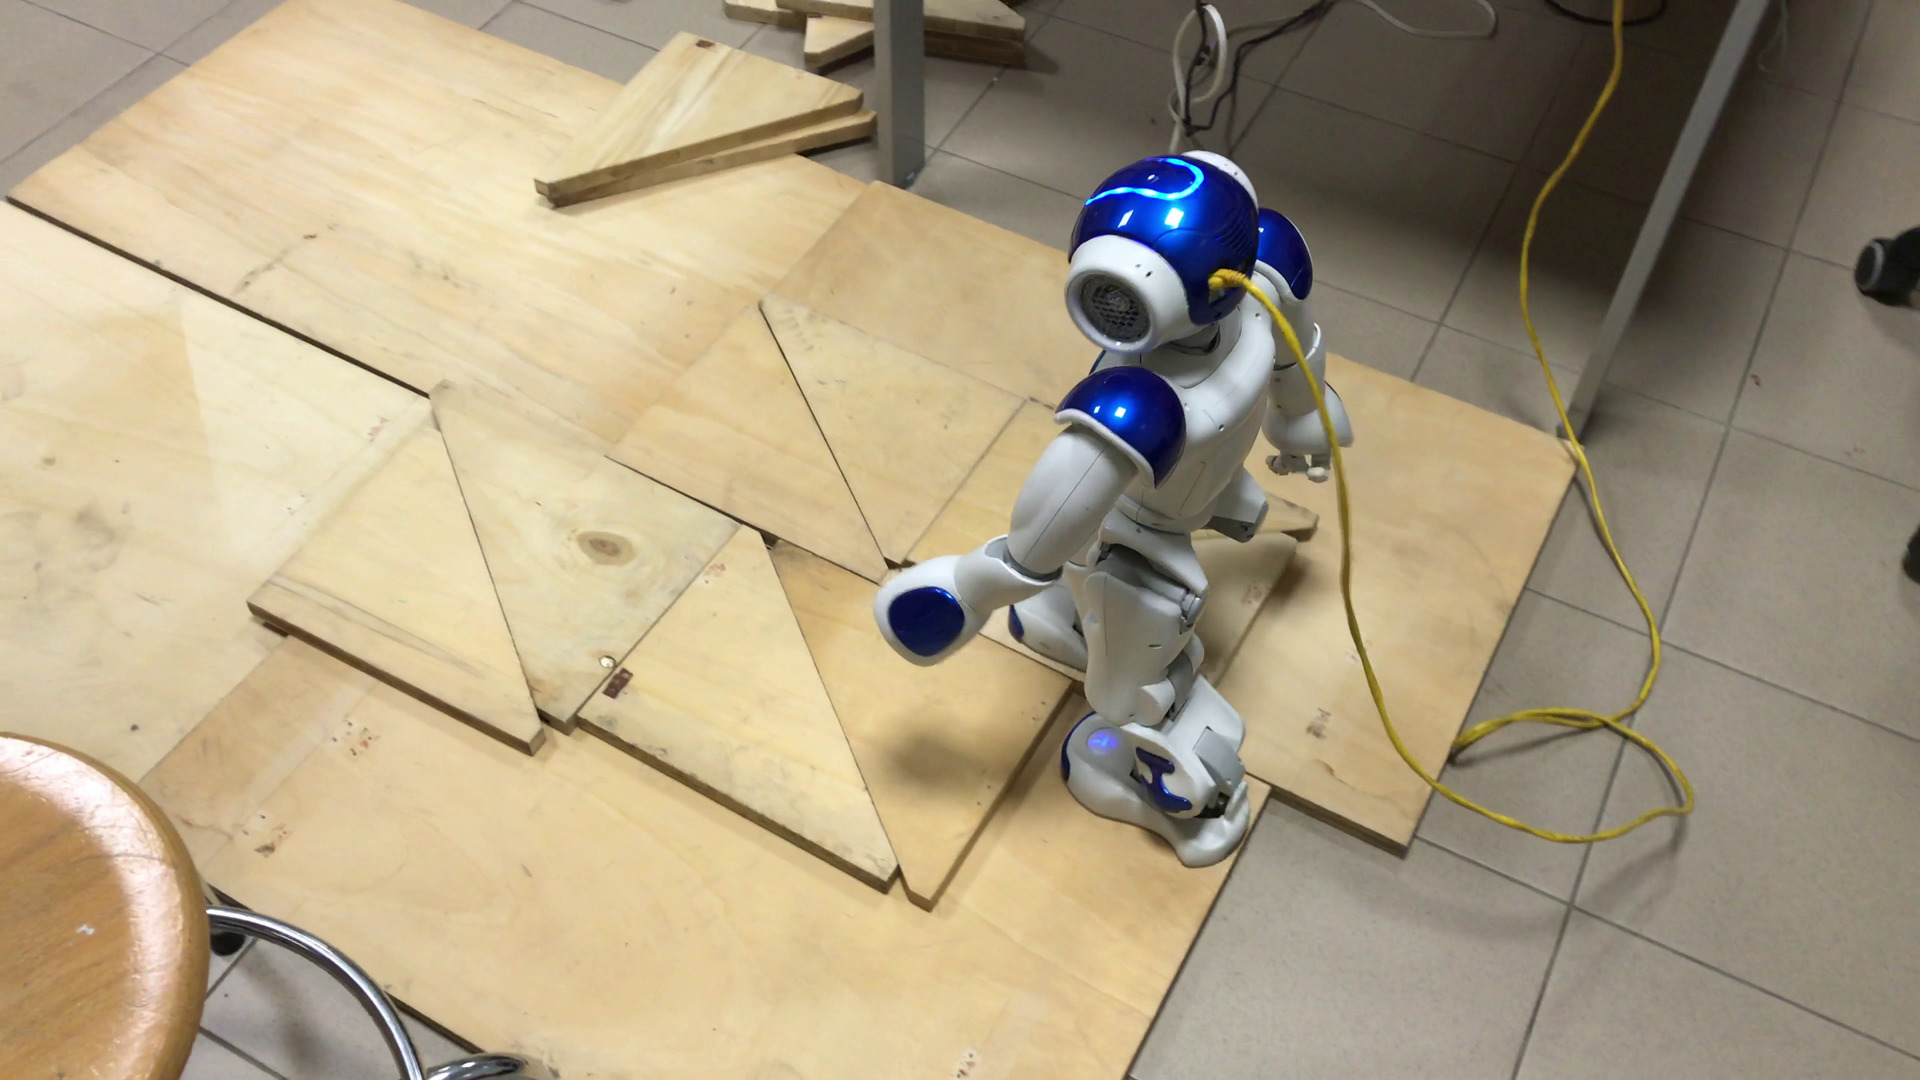
\includegraphics[width=\linewidth]
      {figures/experiments/multiple-staircases/upstairs/video/05.png}
    \caption{Fourth step}
  \end{subfigure}\hspace*{\fill}
  \begin{subfigure}{0.48\textwidth}
    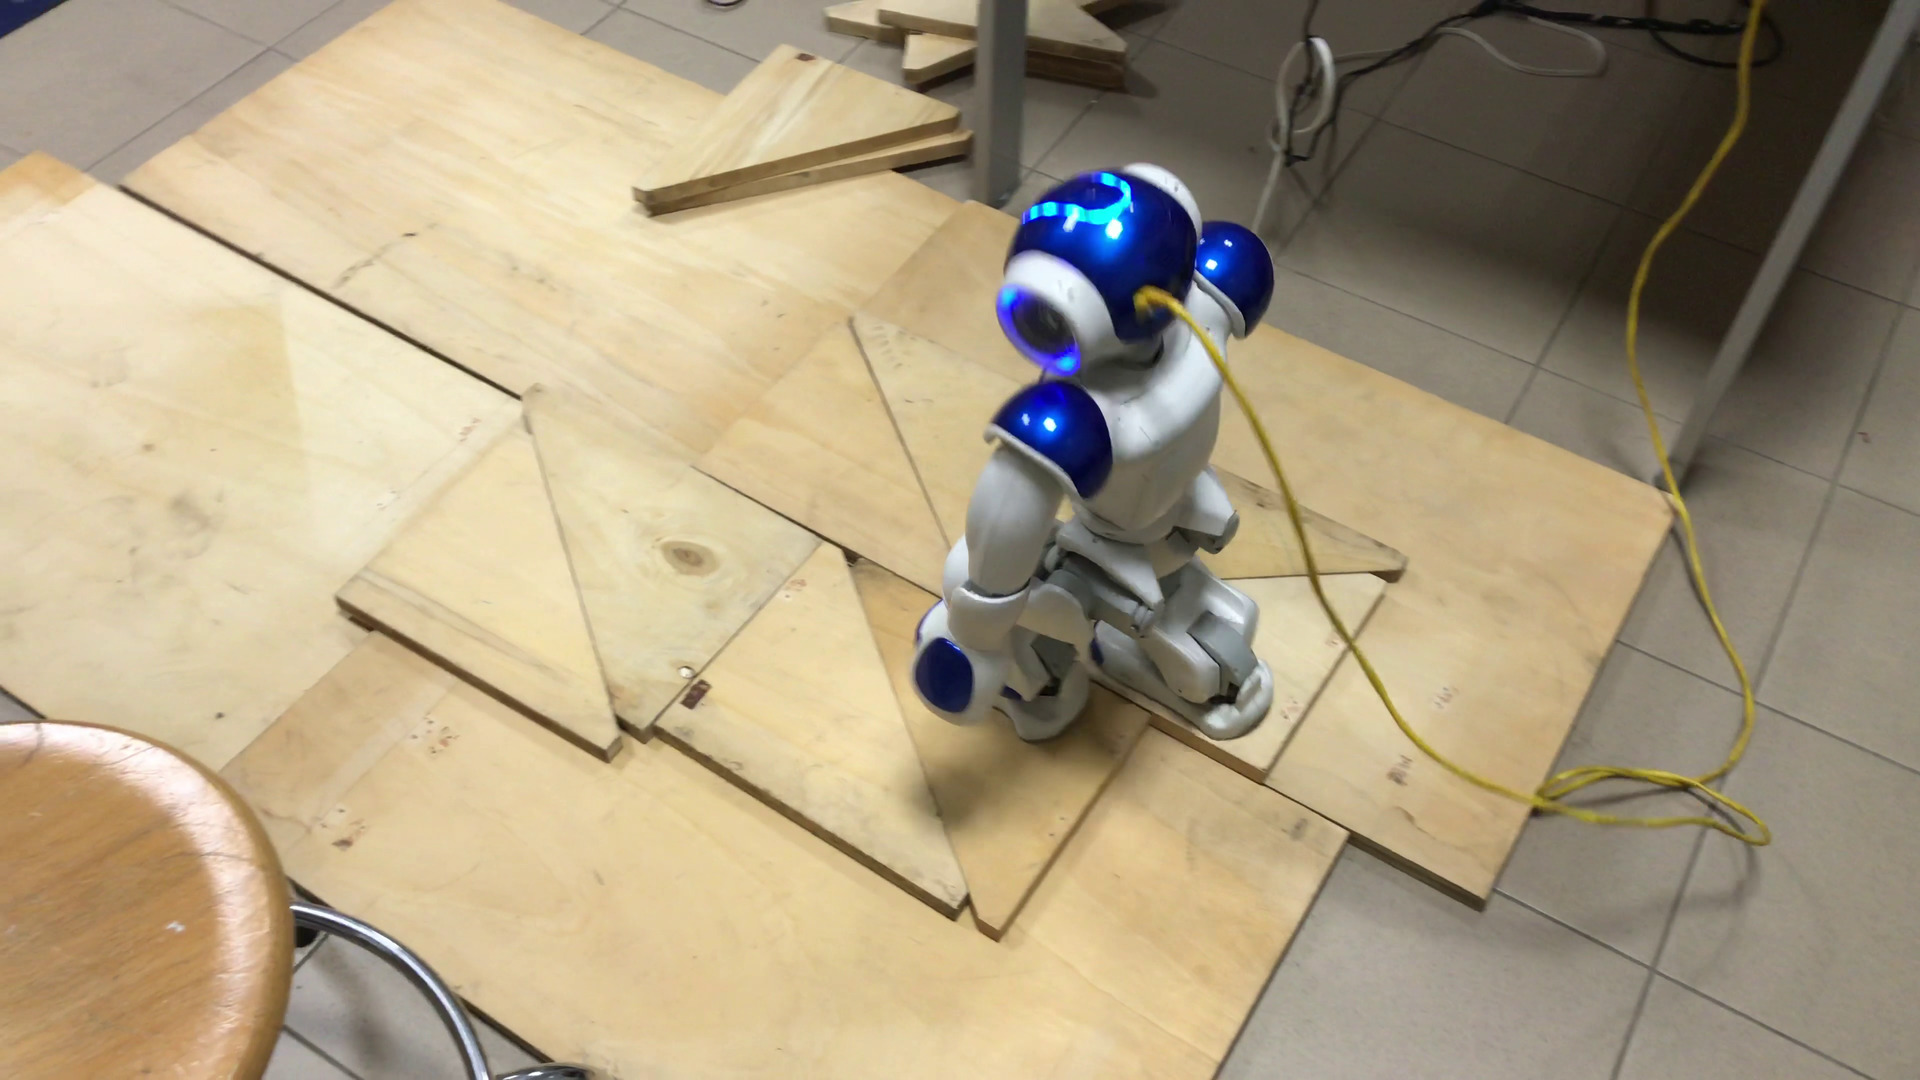
\includegraphics[width=\linewidth]
      {figures/experiments/multiple-staircases/upstairs/video/06.png}
    \caption{Fifth step}
  \end{subfigure}
  \caption{The figures show the motion of the robot for the scenario
      ``Multiple Staircases (Upstairs)''. The robot starts just in 
      front of the stairs (Fig. \ref{fig:exp:ms:up:frame1}), then it places 
      each step one in front of the other without colliding with the staircases,
      safely climbing the stairway. Each staircase has a height of 2 cm.}
  \label{fig:experiments:multiple-staircases:upstairs:videoframes}
\end{figure}

\begin{figure}
  \centering
  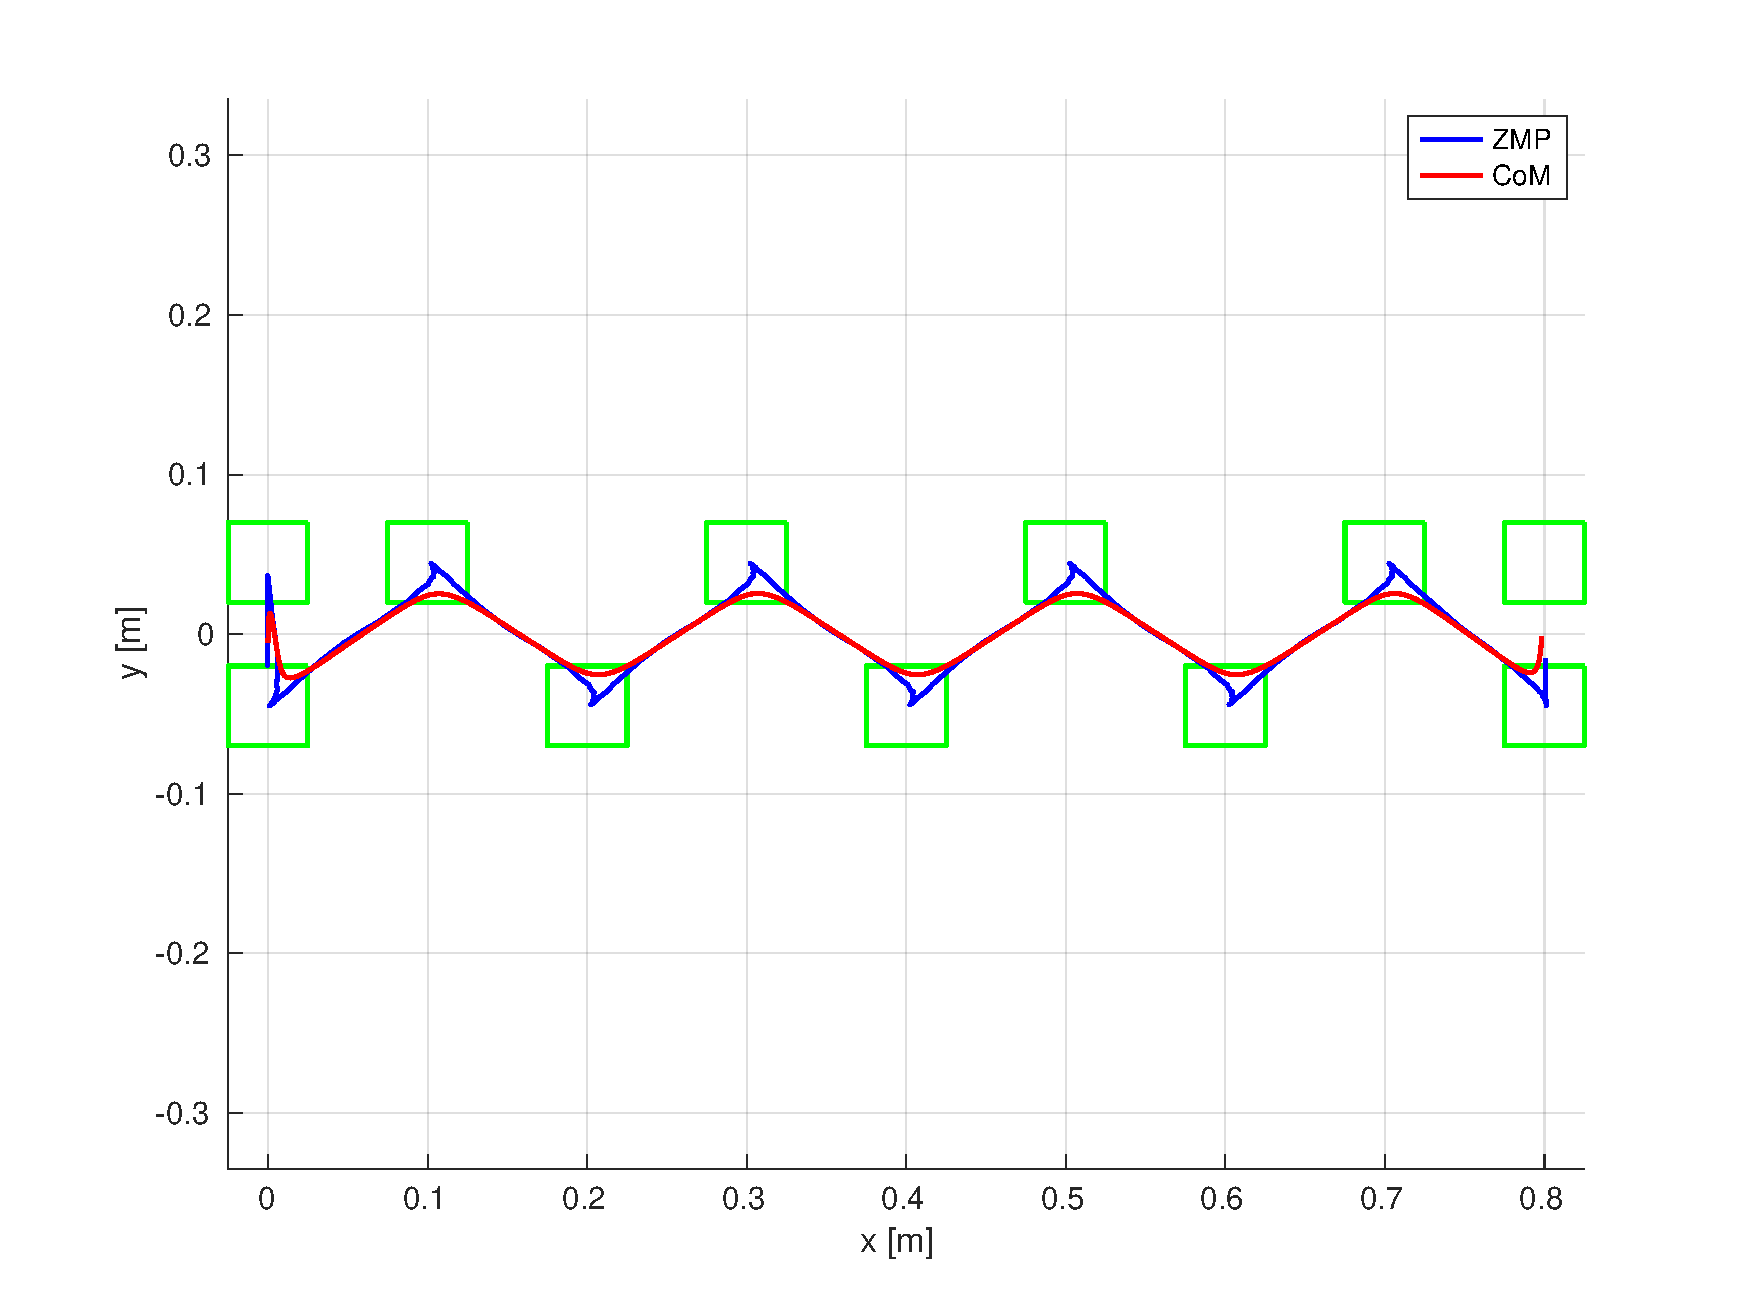
\includegraphics[width=\textwidth]
      {figures/experiments/multiple-staircases/upstairs/xy-plot-2cm.pdf}
  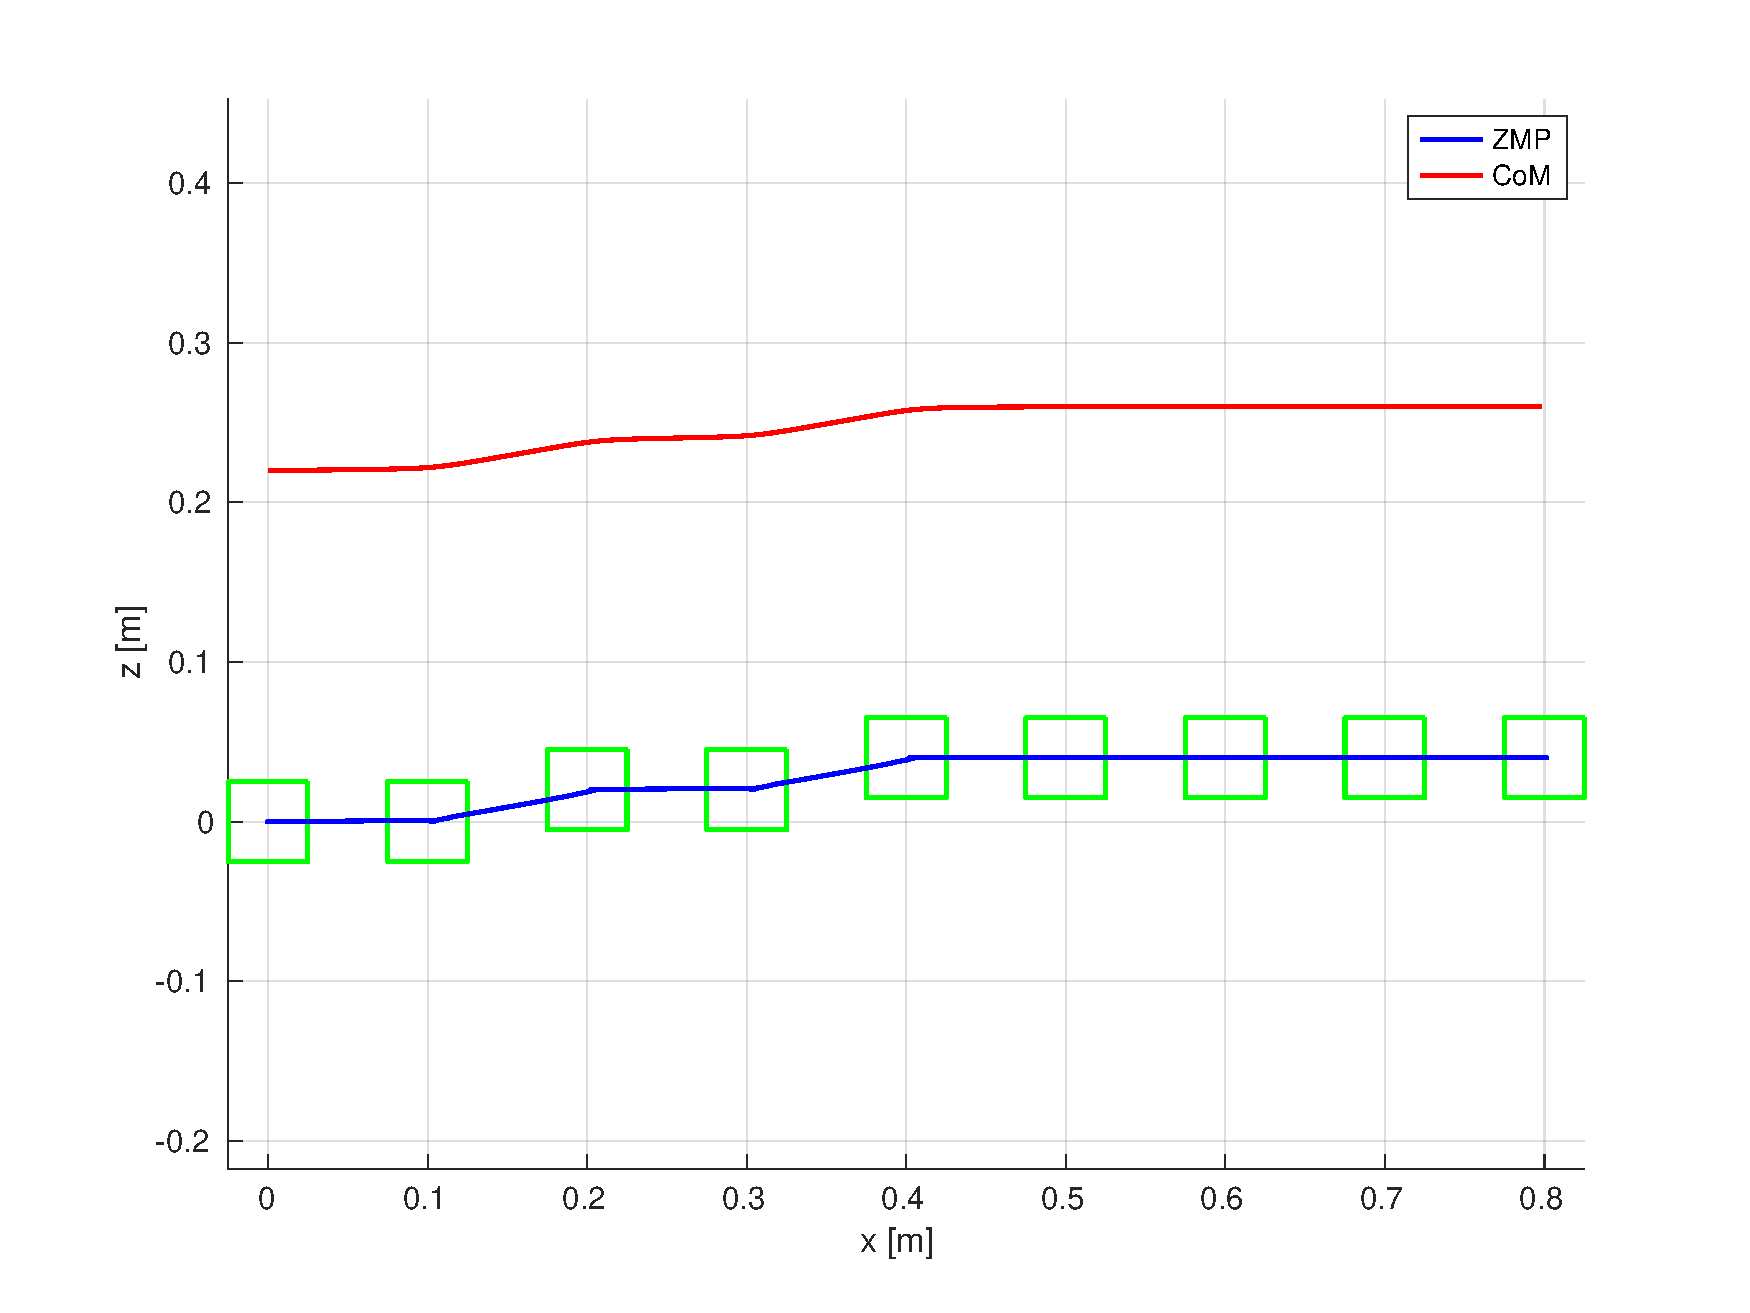
\includegraphics[width=\textwidth]
      {figures/experiments/multiple-staircases/upstairs/xz-plot-2cm.pdf}
  \caption{The plots show how the CoM and the ZMP vary with respect to the
		footsteps in the scenario ``Multiple Staircases (Upstairs)''.
    The green boxes represent the footsteps.}
  \label{fig:experiments:multiple-staircases:upstairs:comzmp}
\end{figure}

\subsection{Downstairs}
Downstairs.
\begin{figure}
  \begin{subfigure}{0.48\textwidth}
    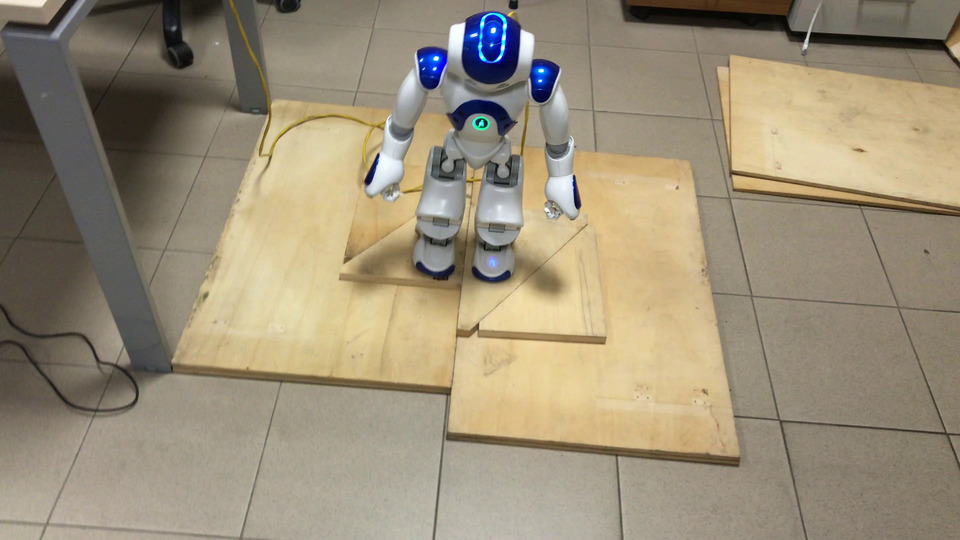
\includegraphics[width=\linewidth]
      {figures/experiments/multiple-staircases/downstairs/video/01.png}
    \caption{Starting position}
    \label{fig:exp:ms:down:frame1}
  \end{subfigure}\hspace*{\fill}
  \begin{subfigure}{0.48\textwidth}
    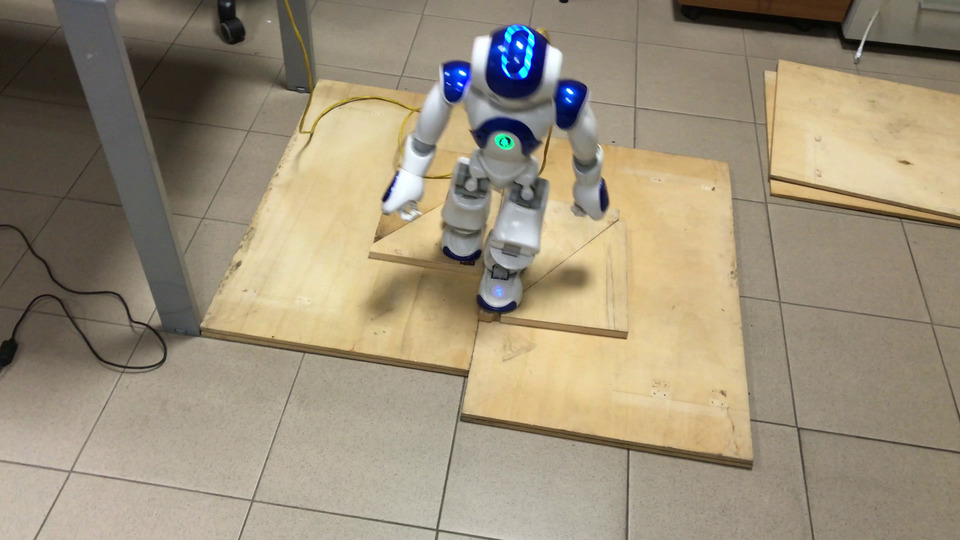
\includegraphics[width=\linewidth]
      {figures/experiments/multiple-staircases/downstairs/video/02.png}
    \caption{First step}
  \end{subfigure}
  \begin{subfigure}{0.48\textwidth}
    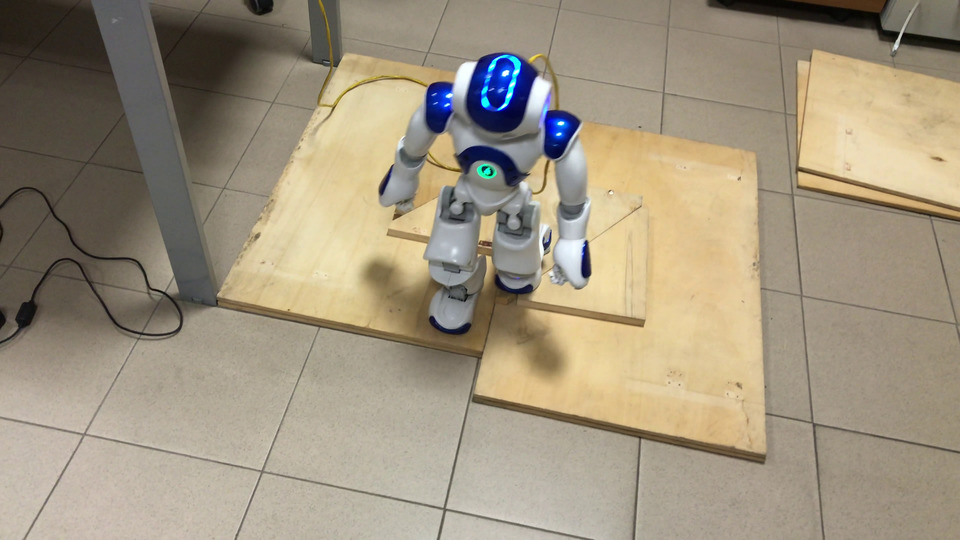
\includegraphics[width=\linewidth]
      {figures/experiments/multiple-staircases/downstairs/video/03.png}
    \caption{Second step}
  \end{subfigure}\hspace*{\fill}
  \begin{subfigure}{0.48\textwidth}
    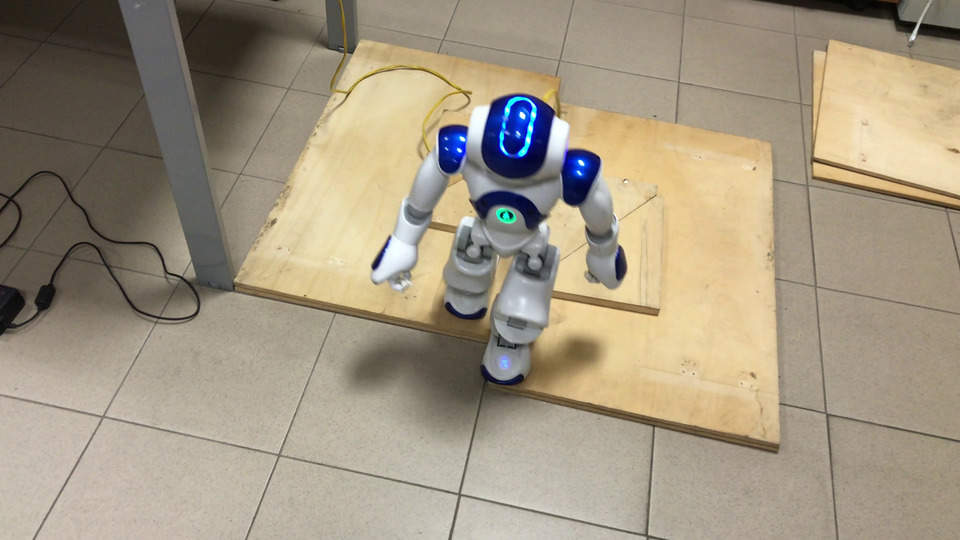
\includegraphics[width=\linewidth]
      {figures/experiments/multiple-staircases/downstairs/video/04.png}
    \caption{Third step}
  \end{subfigure}
  \begin{subfigure}{0.48\textwidth}
    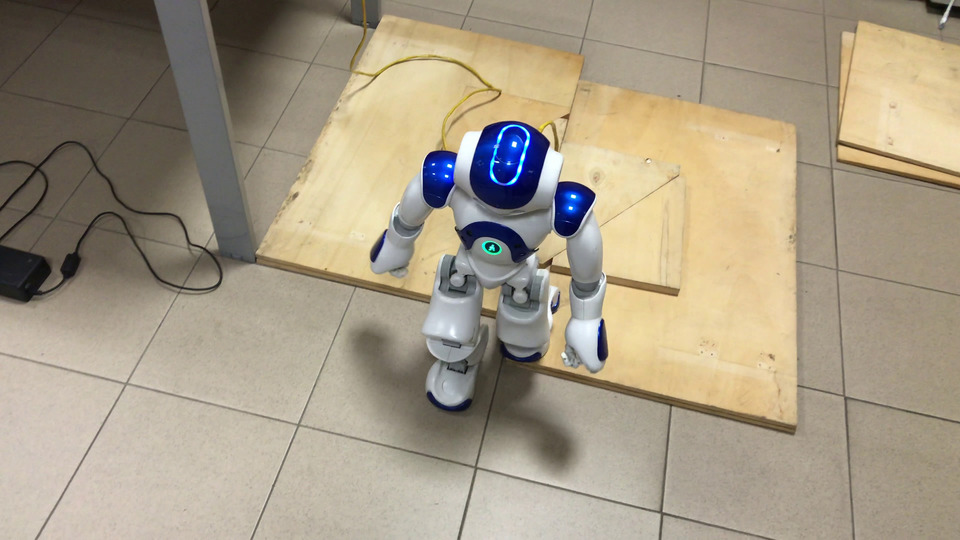
\includegraphics[width=\linewidth]
      {figures/experiments/multiple-staircases/downstairs/video/05.png}
    \caption{Fourth step}
  \end{subfigure}\hspace*{\fill}
  \begin{subfigure}{0.48\textwidth}
    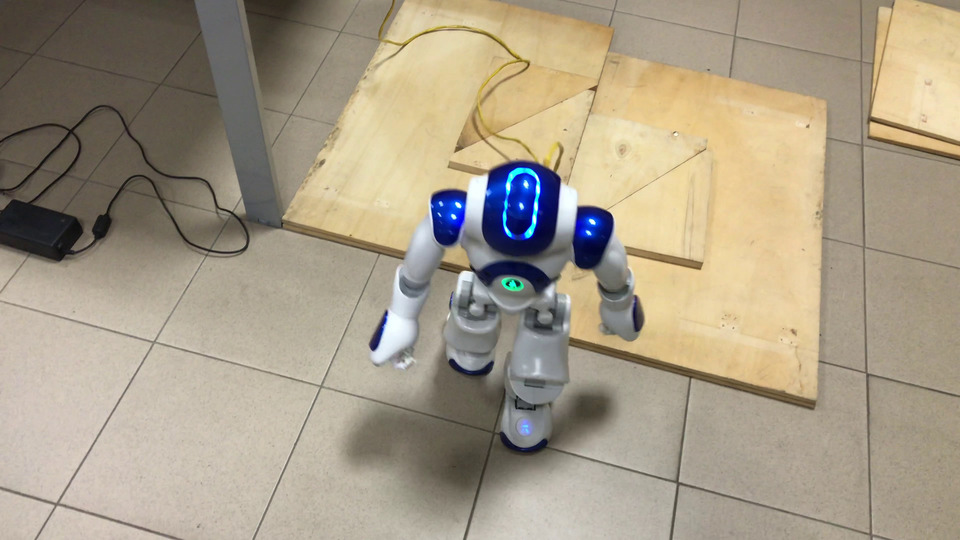
\includegraphics[width=\linewidth]
      {figures/experiments/multiple-staircases/downstairs/video/06.png}
    \caption{Fifth step}
  \end{subfigure}
  \caption{The figures show the motion of the robot for the scenario
      ``Multiple Staircases (Downstairs)''. The robot starts on top of the 
      stairway (Fig. \ref{fig:exp:ms:down:frame1}), then it places 
      each step one in front of the other without colliding with the staircases,
      safely reaching ground level. Each staircase has a height of 2 cm.}
  \label{fig:experiments:multiple-staircases:downstairs:videoframes}
\end{figure}

\begin{figure}
  \centering
  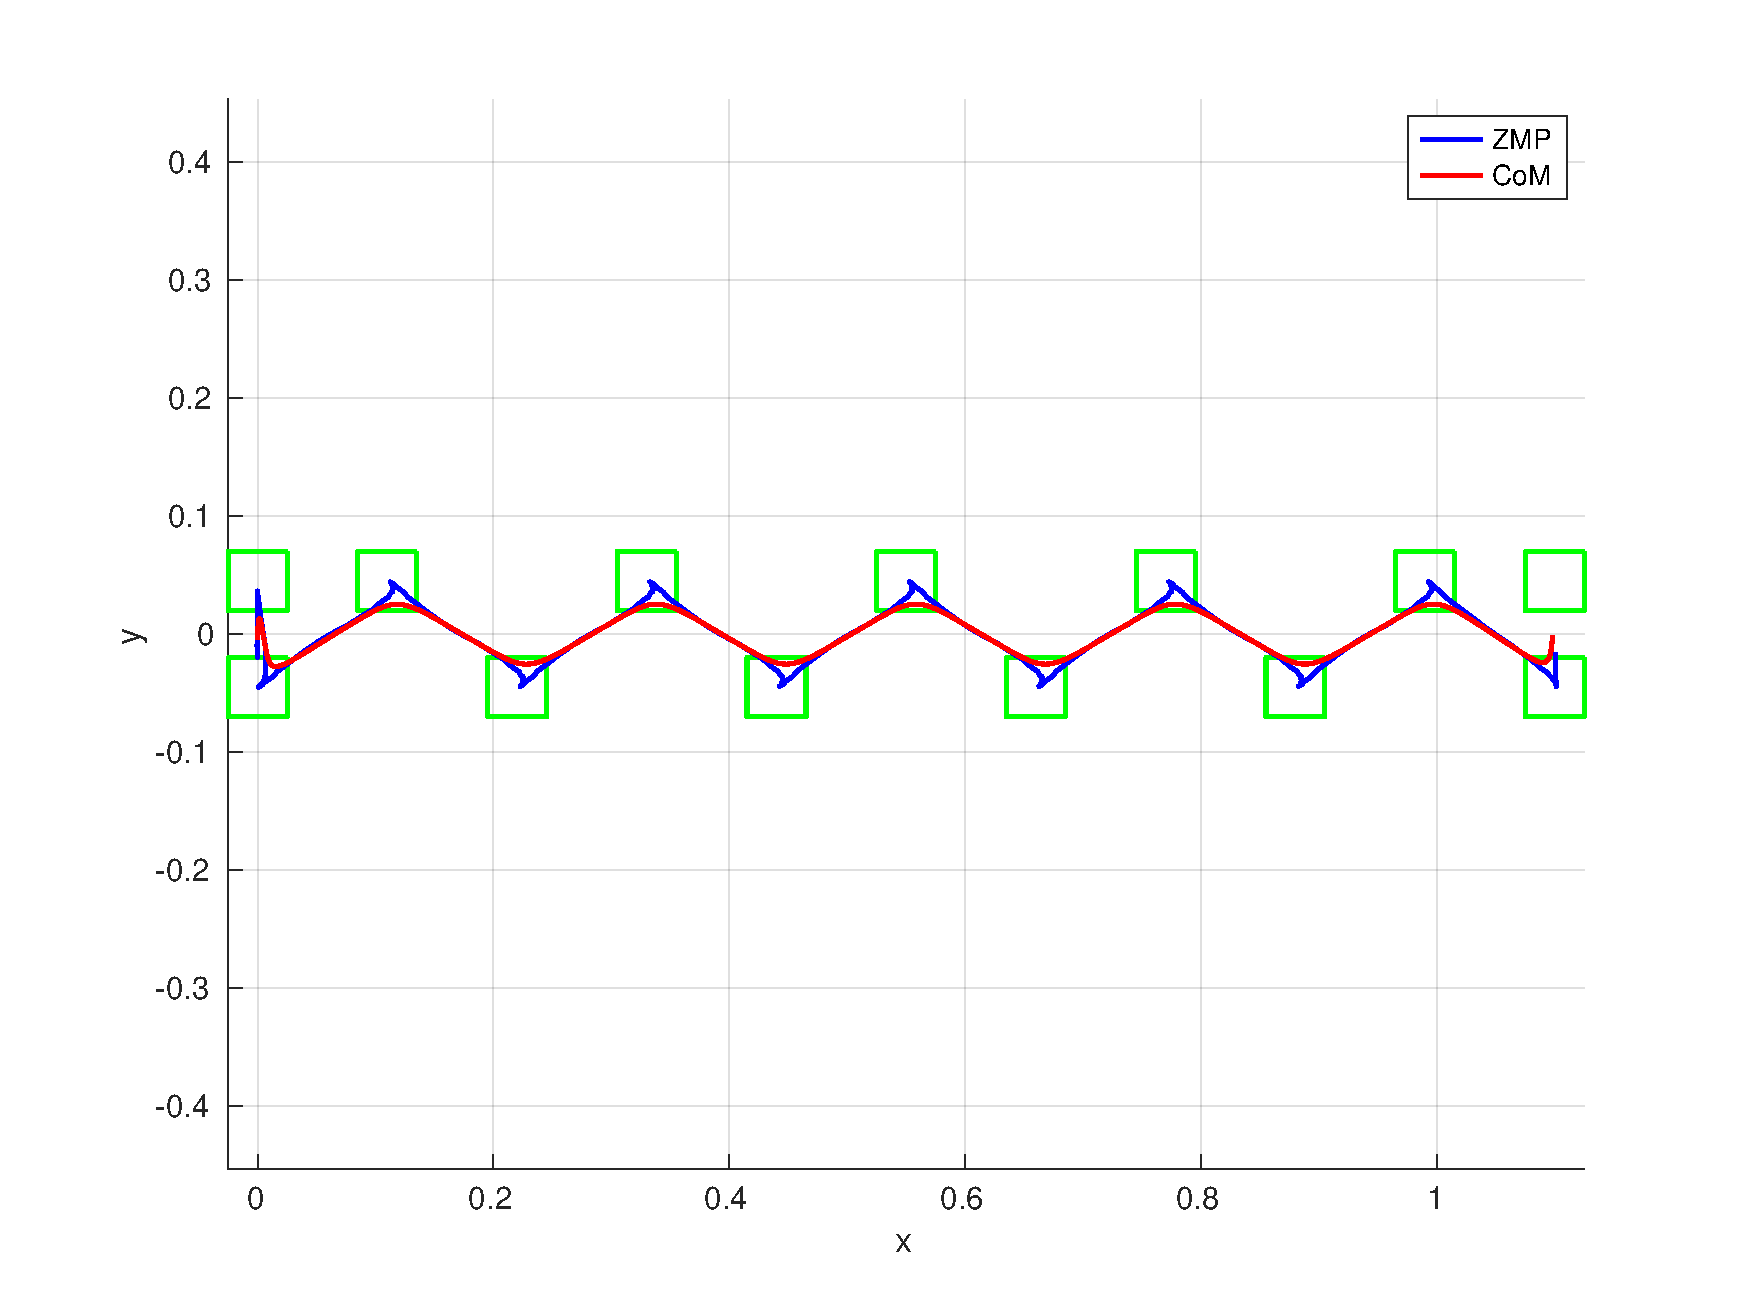
\includegraphics[width=\textwidth]
      {figures/experiments/multiple-staircases/downstairs/xy-plot-2cm.pdf}
  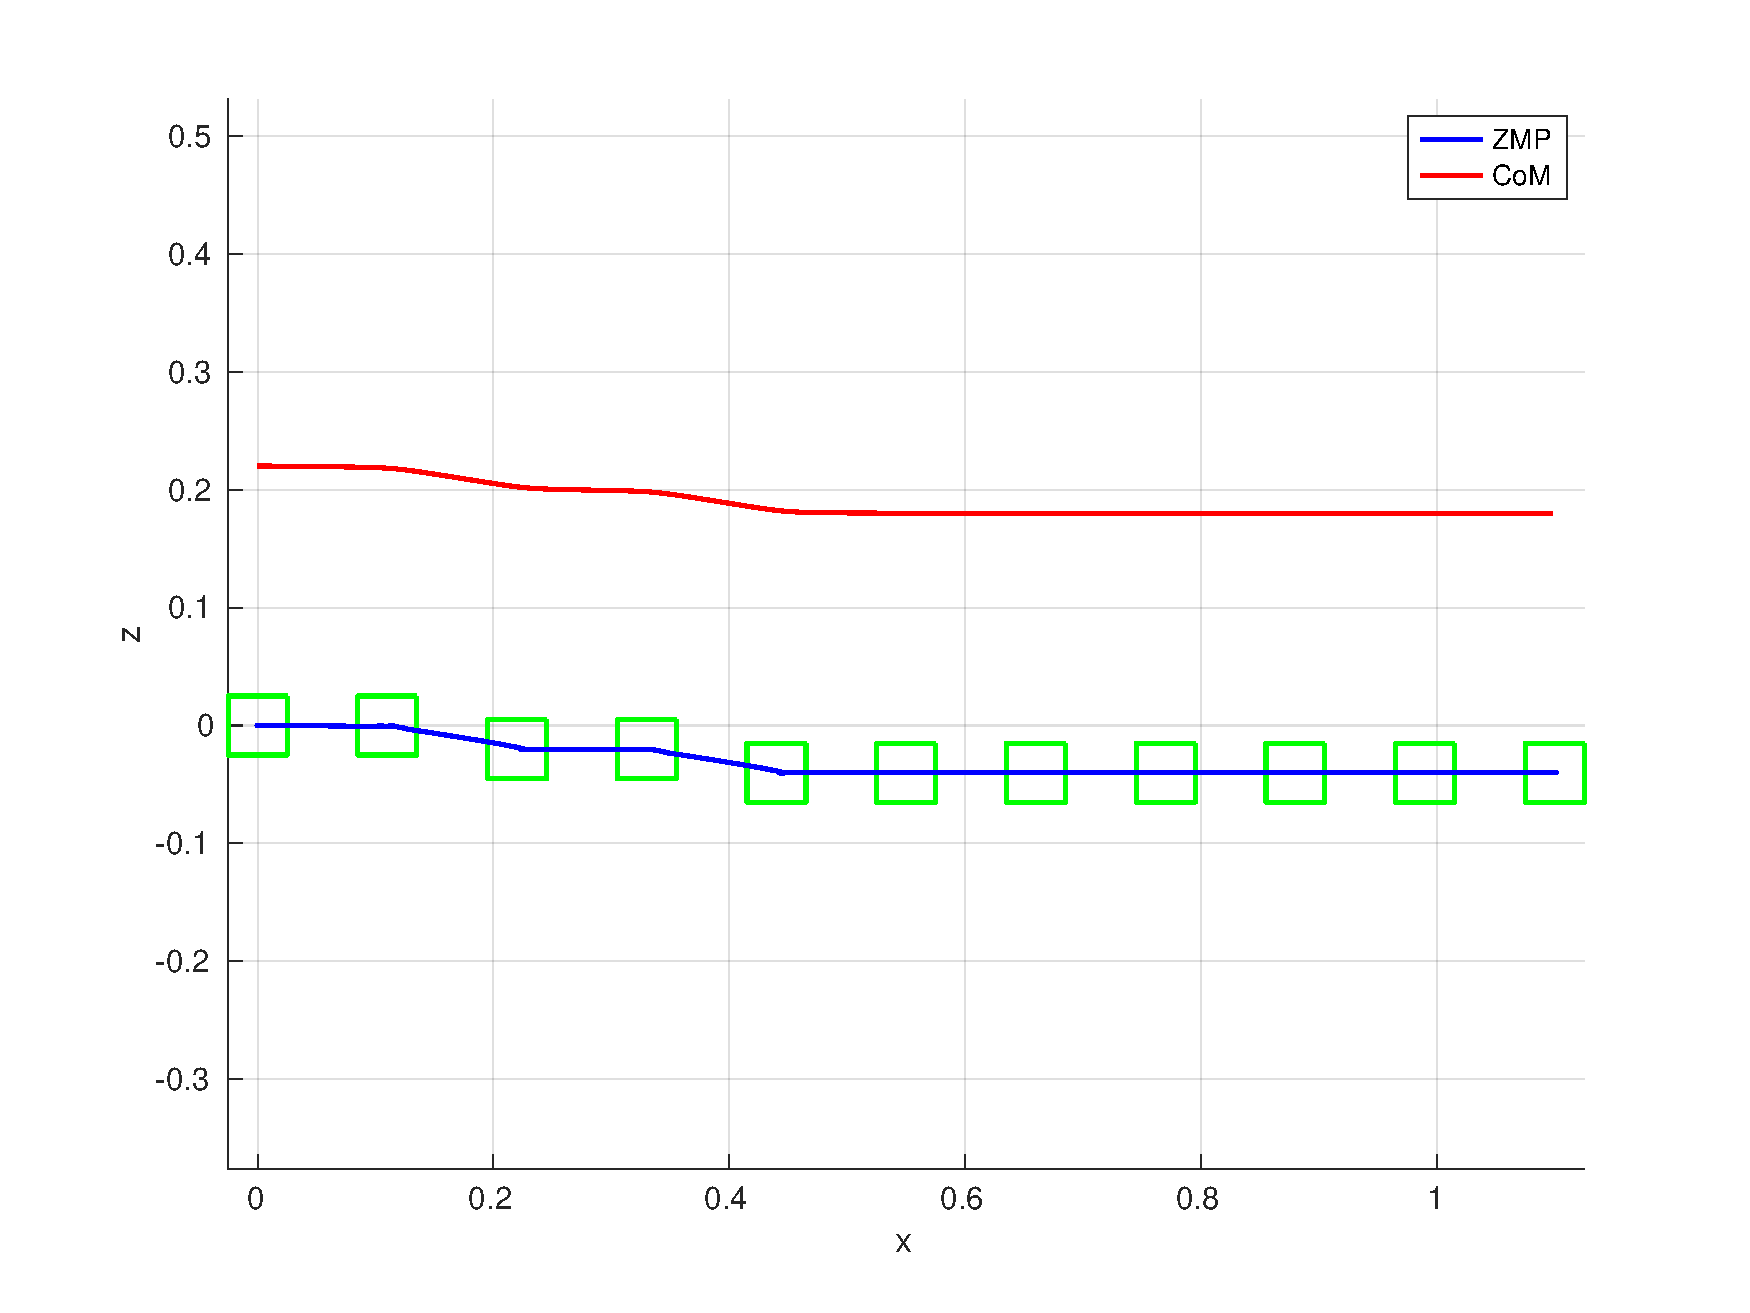
\includegraphics[width=\textwidth]
      {figures/experiments/multiple-staircases/downstairs/xz-plot-2cm.pdf}
  \caption{The plots show how the CoM and the ZMP vary with respect to the
		footsteps in the scenario ``Multiple Staircases (Downstairs)''.
    The green boxes represent the footsteps.}
  \label{fig:experiments:multiple-staircases:downstairs:comzmp}
\end{figure}

\section{Obstacle Avoidance}
Footstep planning with manually generated elevation mapping. Map contains 
an obstacle that can not be climbed by NAO because of short legs.
\begin{figure}
    \centering
    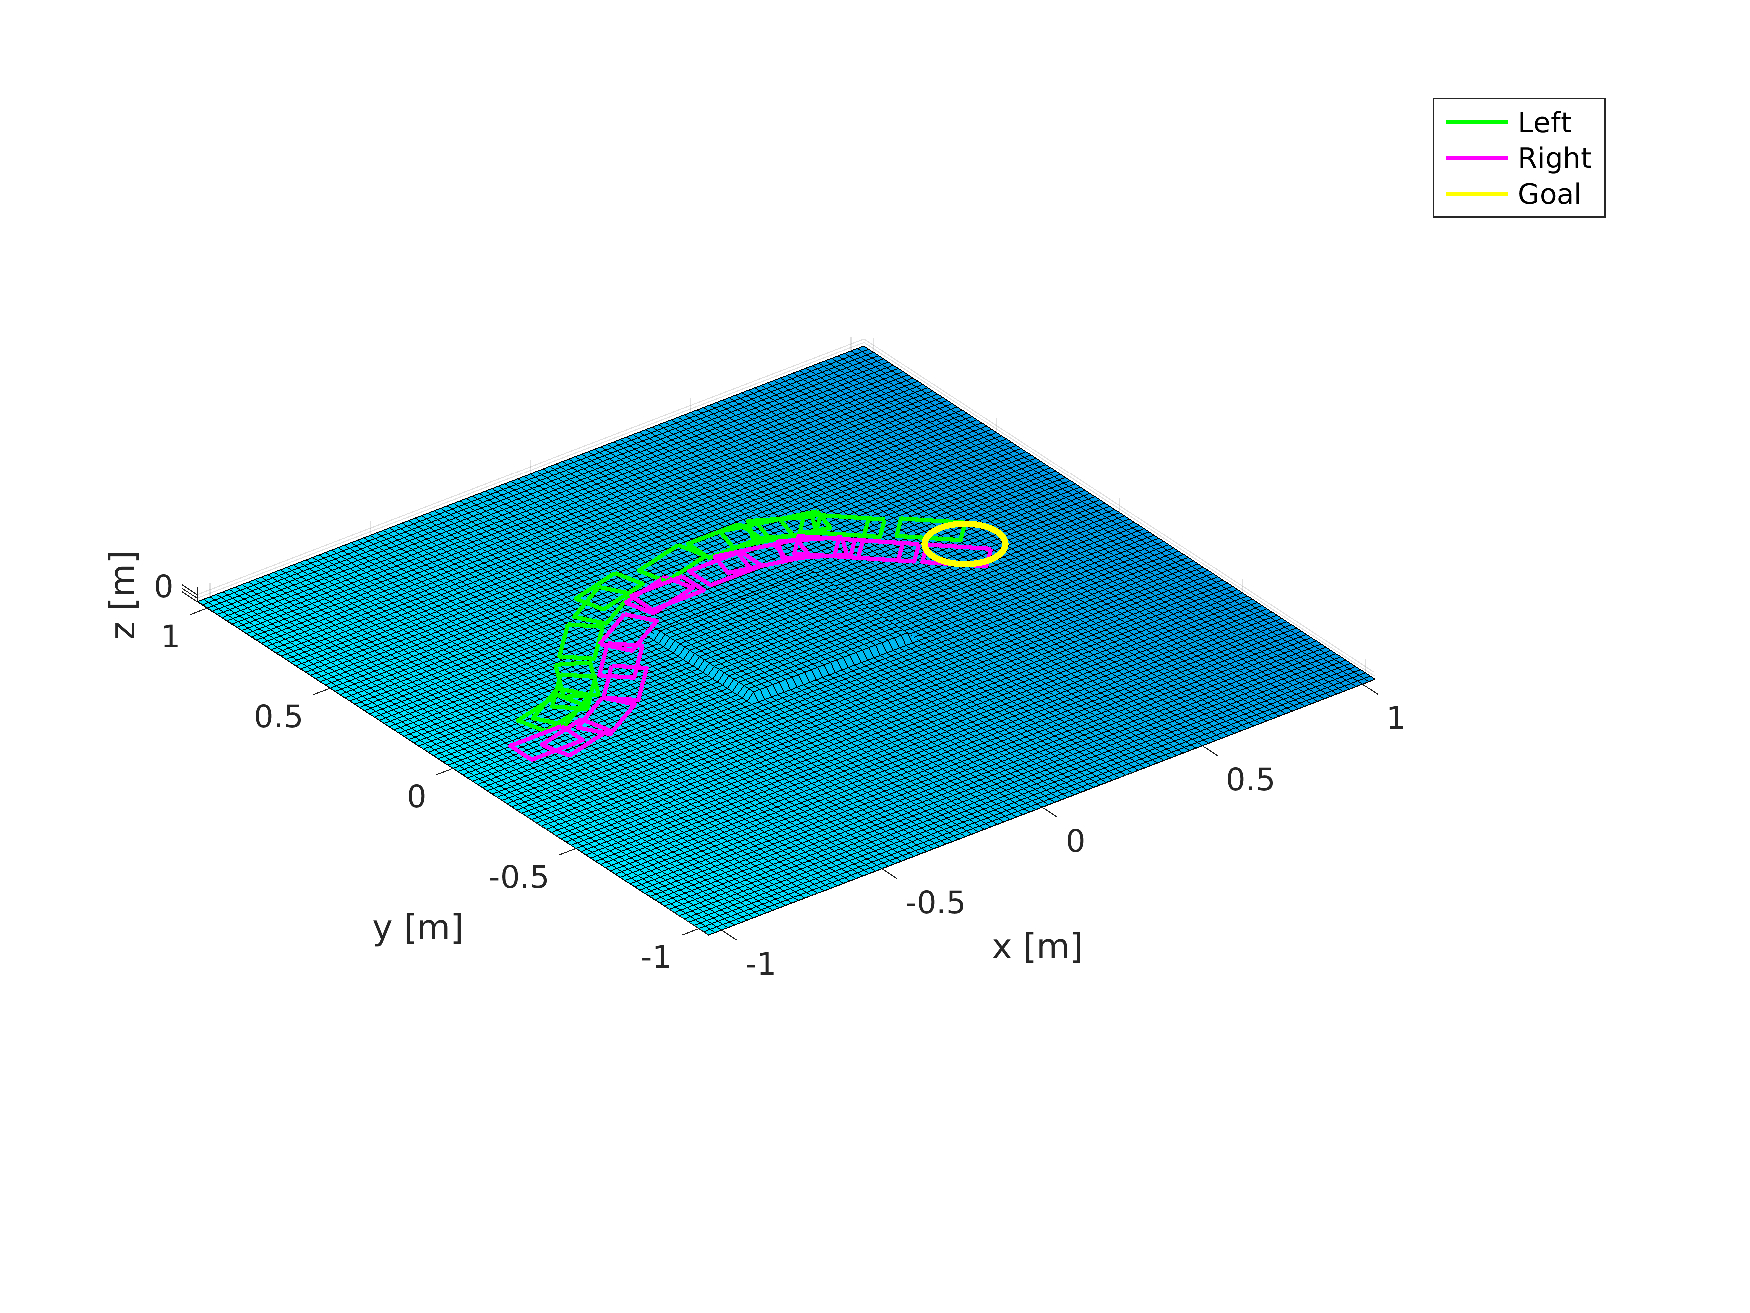
\includegraphics[width=0.95\textwidth]
        {figures/experiments/obstacle-avoidance/footstep-plan.pdf}
    \caption{Footstep plan generated for the scenario ``Obstacle Avoidance''.}
    \label{fig:experiments:obstacle-avoidance:footstep-plan}
\end{figure}
\begin{figure}
    \centering
    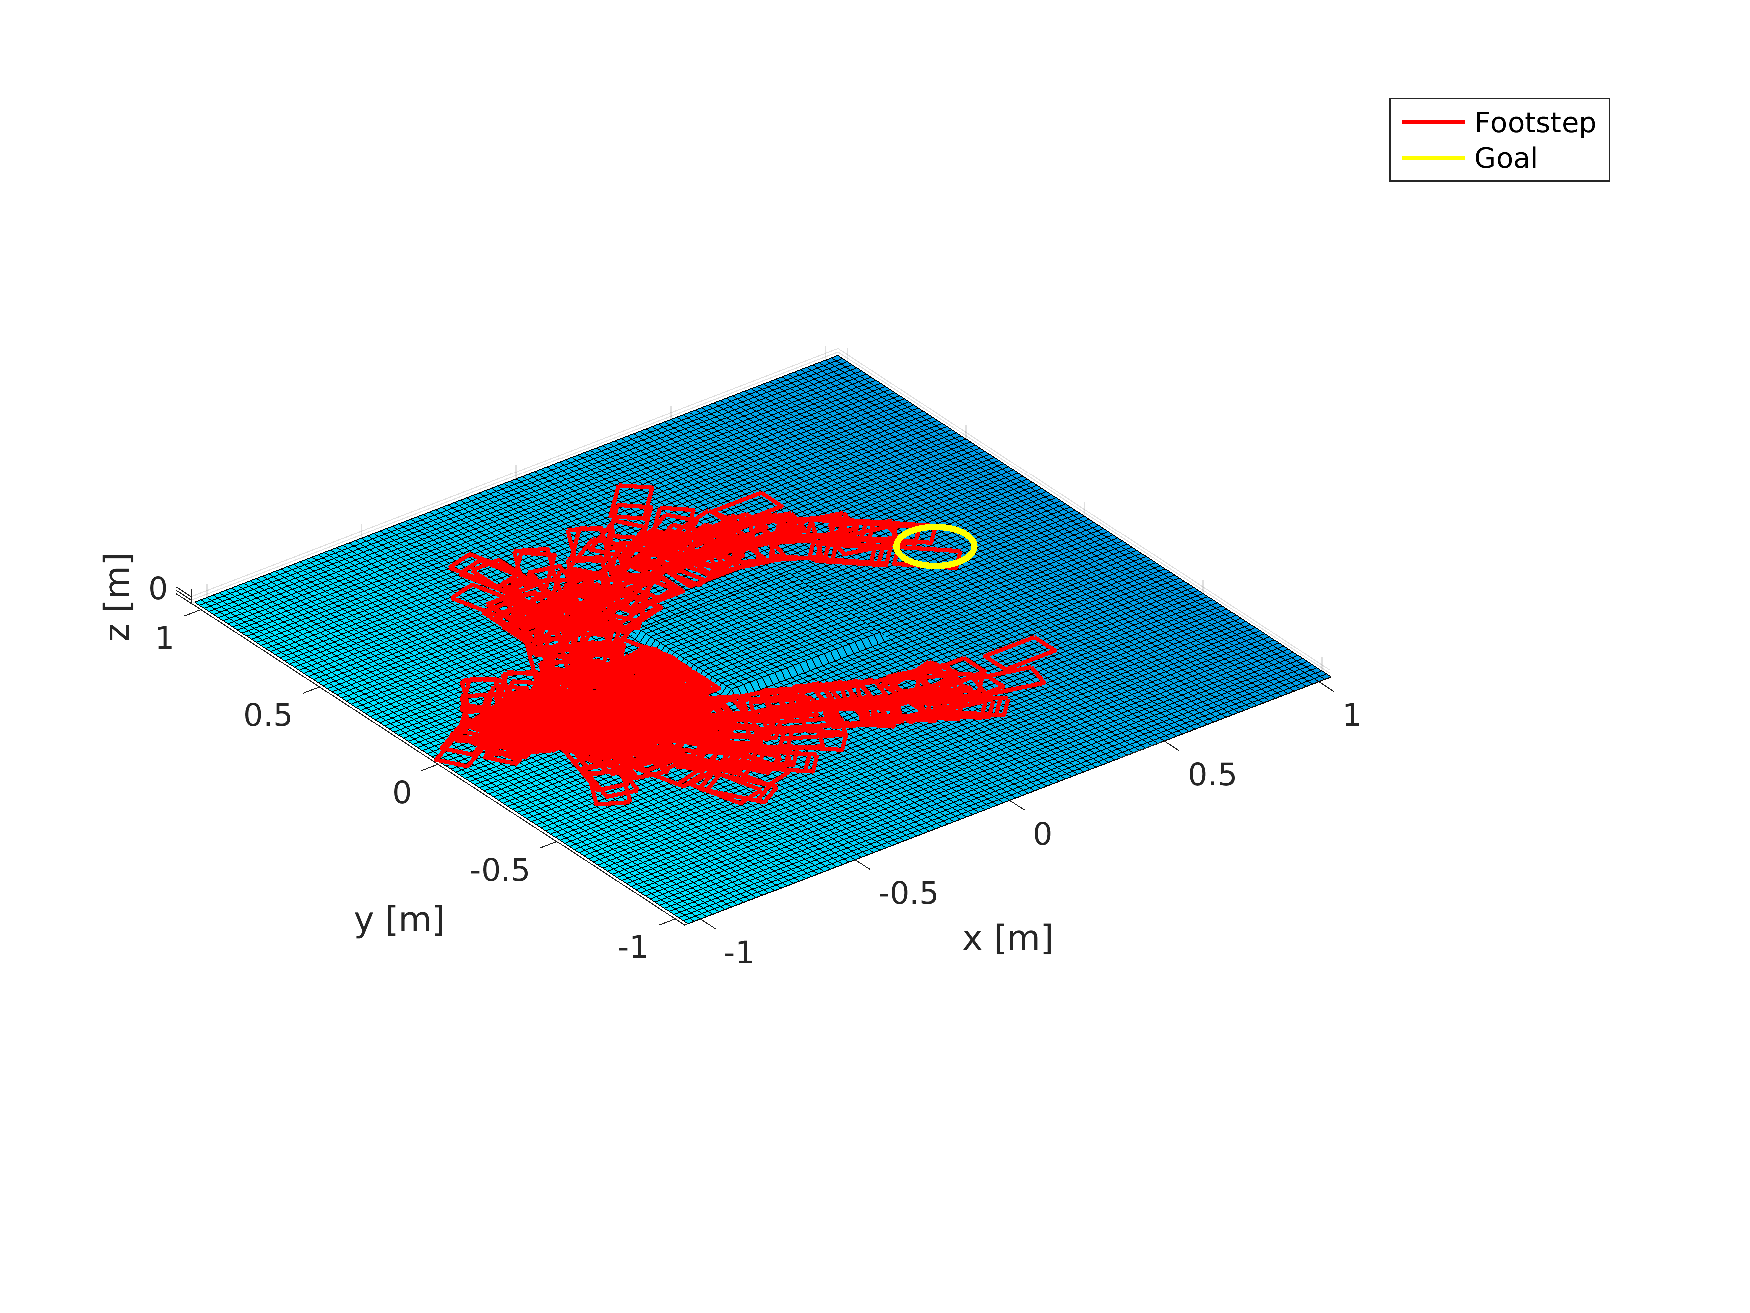
\includegraphics[width=0.95\textwidth]
        {figures/experiments/obstacle-avoidance/rrt-tree.pdf}
    \caption{Tree generated for the scenario ``Obstacle Avoidance''.}
    \label{fig:experiments:obstacle-avoidance:rrt-tree}
\end{figure}

\section{Stair Climbing in Unknown Environment}
Stair climbing (unknown environment). Planner + \texttt{elevation\_mapping}.
\begin{figure}
  \begin{subfigure}{0.48\textwidth}
    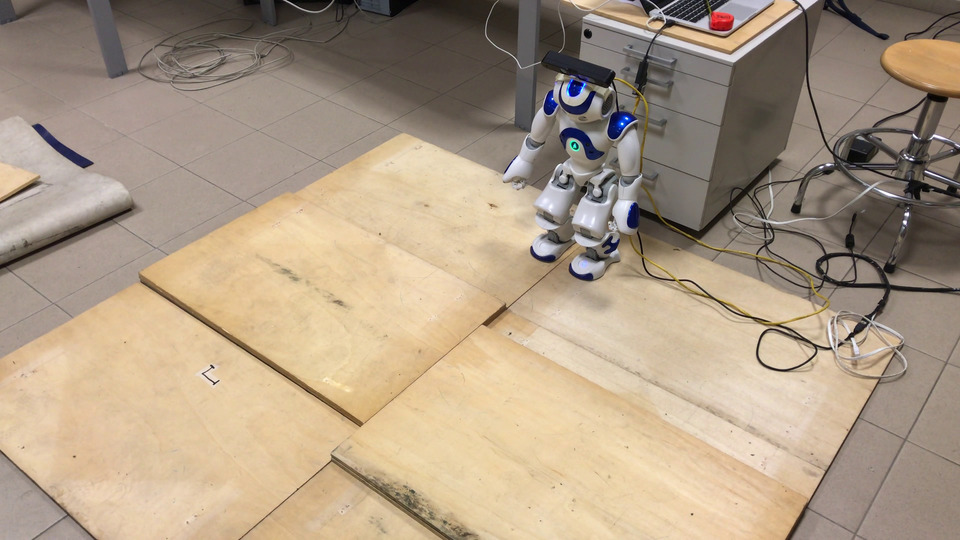
\includegraphics[width=\linewidth]
      {figures/experiments/unknown-env/video/01.png}
    \caption{Starting position}
    \label{fig:exp:unkenv:frame1}
  \end{subfigure}\hspace*{\fill}
  \begin{subfigure}{0.48\textwidth}
    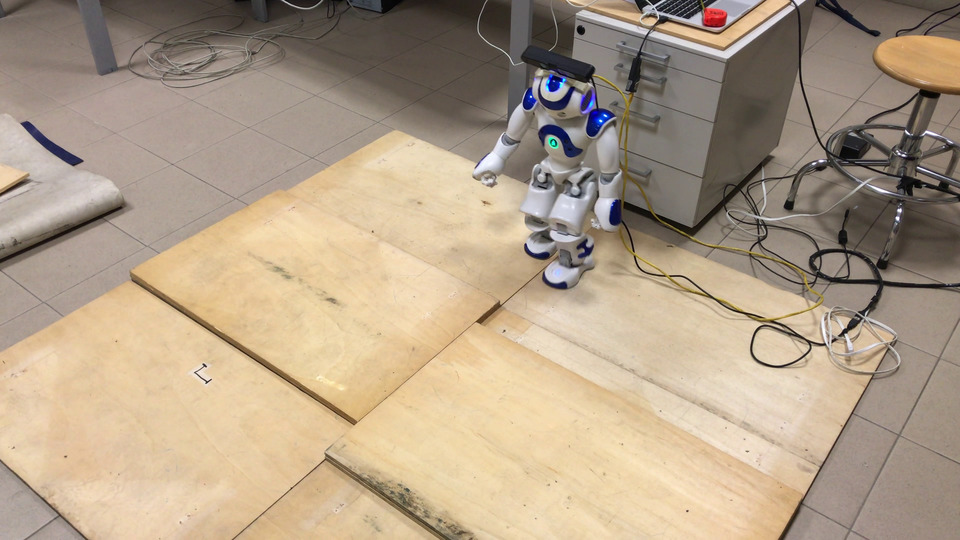
\includegraphics[width=\linewidth]
      {figures/experiments/unknown-env/video/02.png}
    \caption{First step}
    \label{fig:exp:unkenv:frame2}
  \end{subfigure}
  \begin{subfigure}{0.48\textwidth}
    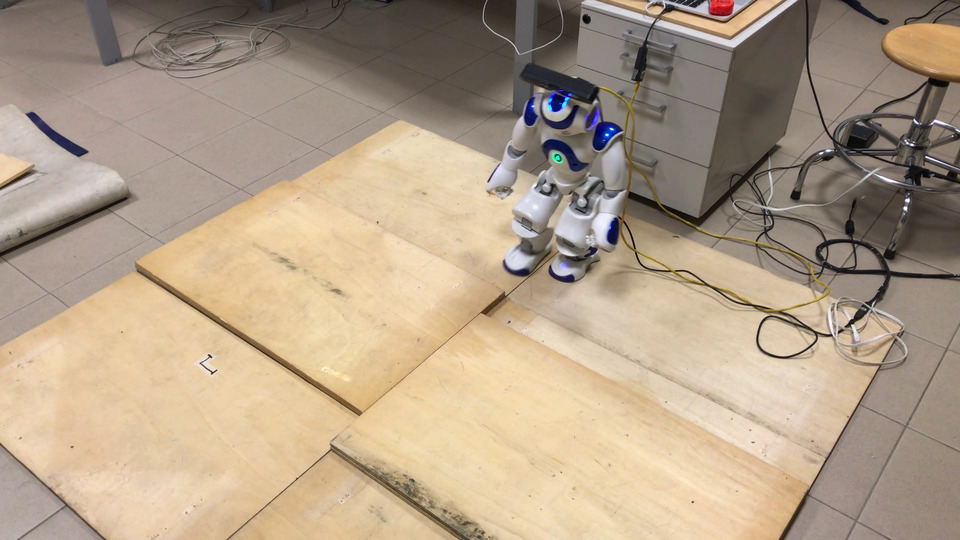
\includegraphics[width=\linewidth]
      {figures/experiments/unknown-env/video/03.png}
    \caption{Second step}
  \end{subfigure}\hspace*{\fill}
  \begin{subfigure}{0.48\textwidth}
    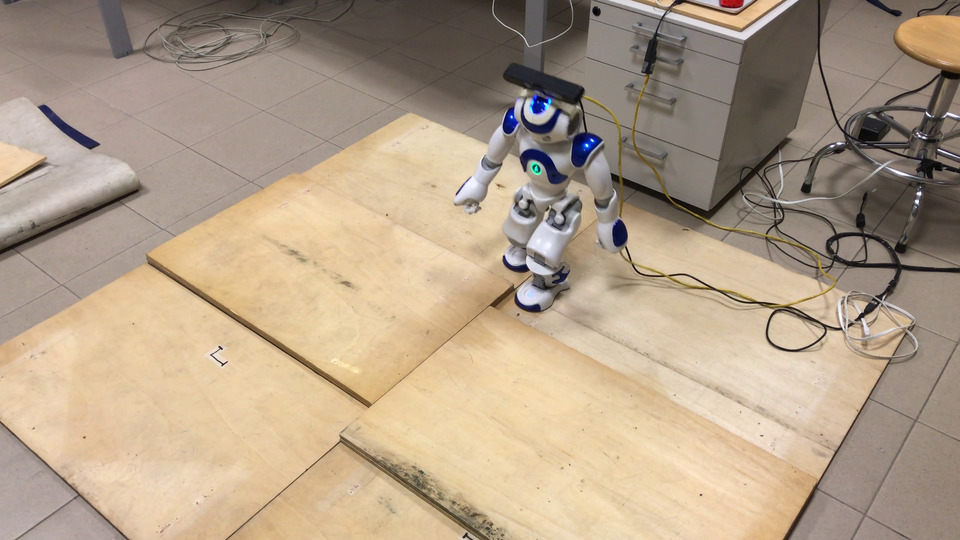
\includegraphics[width=\linewidth]
      {figures/experiments/unknown-env/video/04.png}
    \caption{Third step}
  \end{subfigure}
  \begin{subfigure}{0.48\textwidth}
    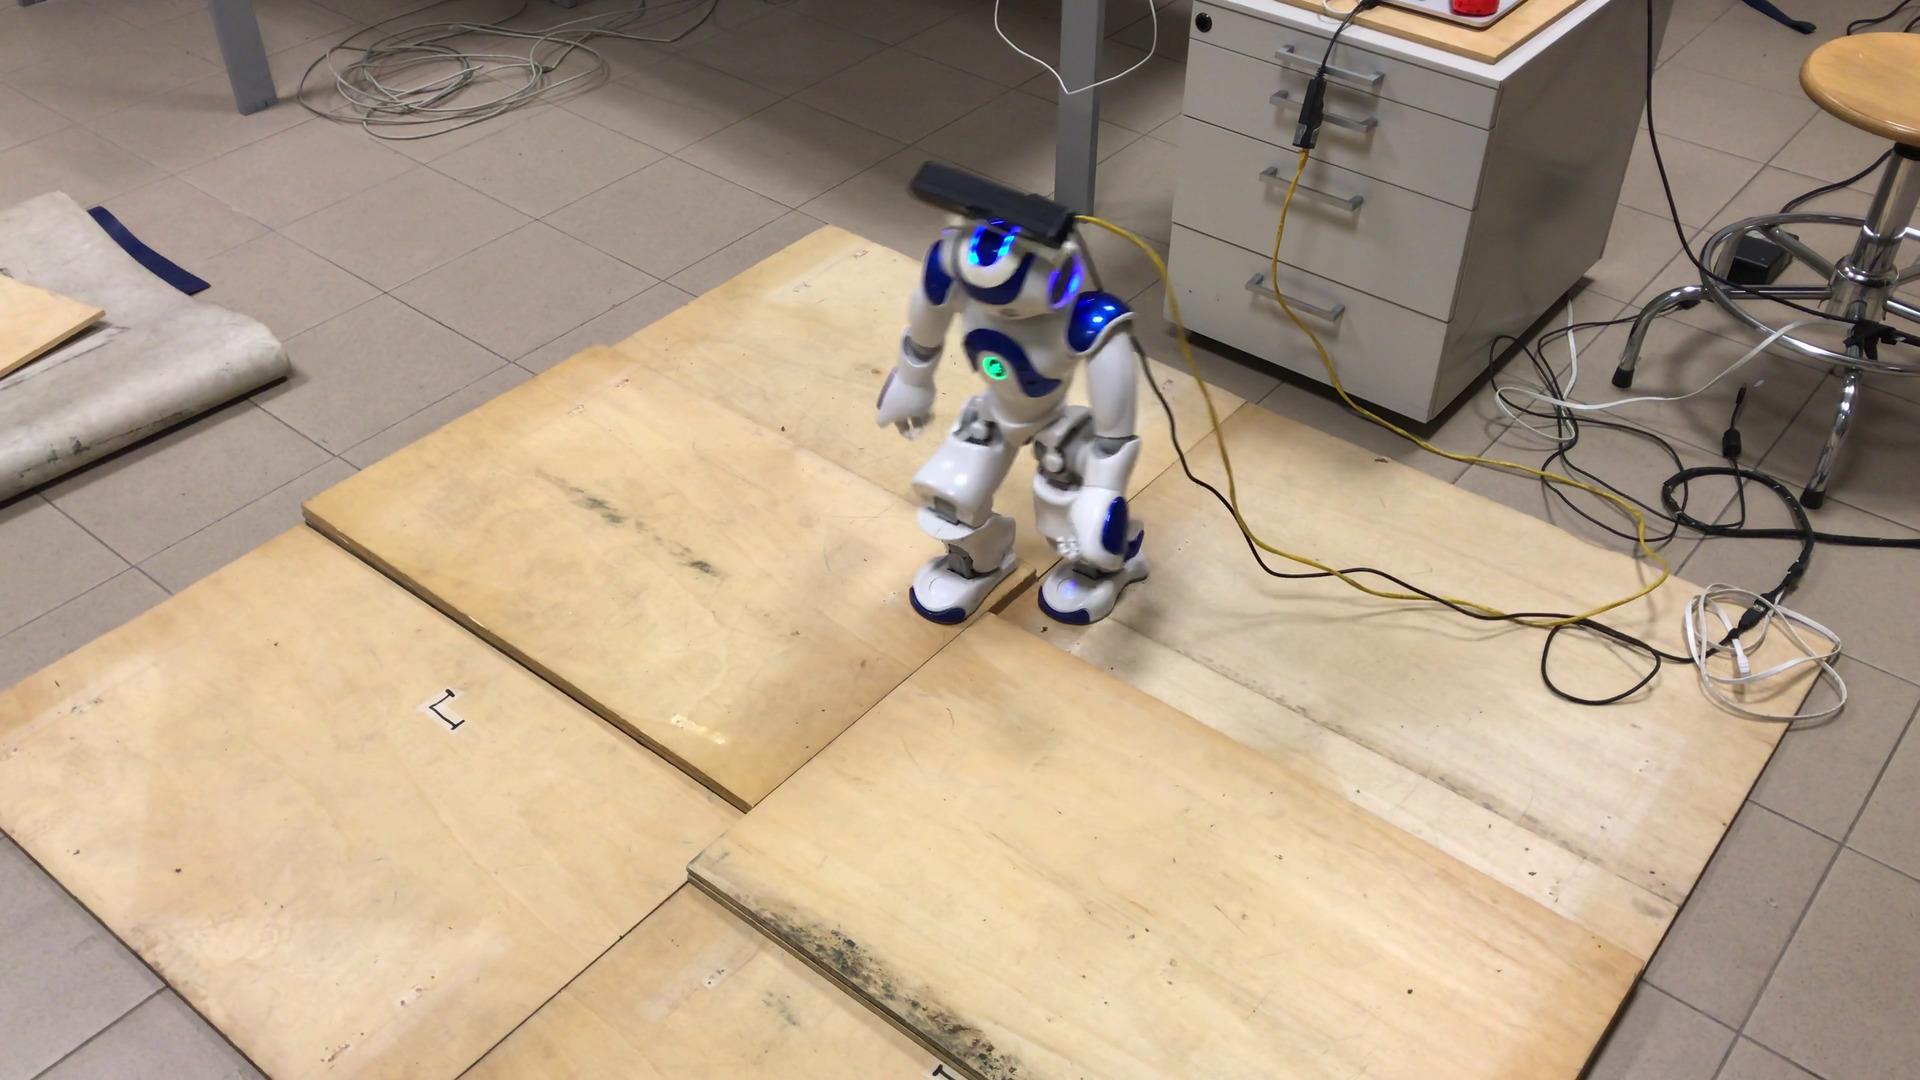
\includegraphics[width=\linewidth]
      {figures/experiments/unknown-env/video/05.png}
    \caption{Fourth step}
  \end{subfigure}\hspace*{\fill}
  \begin{subfigure}{0.48\textwidth}
    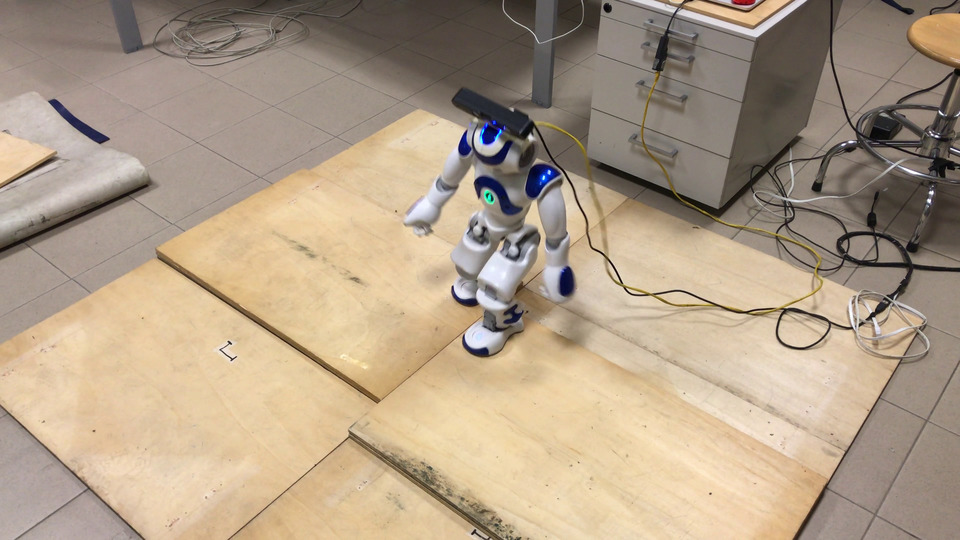
\includegraphics[width=\linewidth]
      {figures/experiments/unknown-env/video/06.png}
    \caption{Fifth step}
  \end{subfigure}
  \begin{subfigure}{0.48\textwidth}
    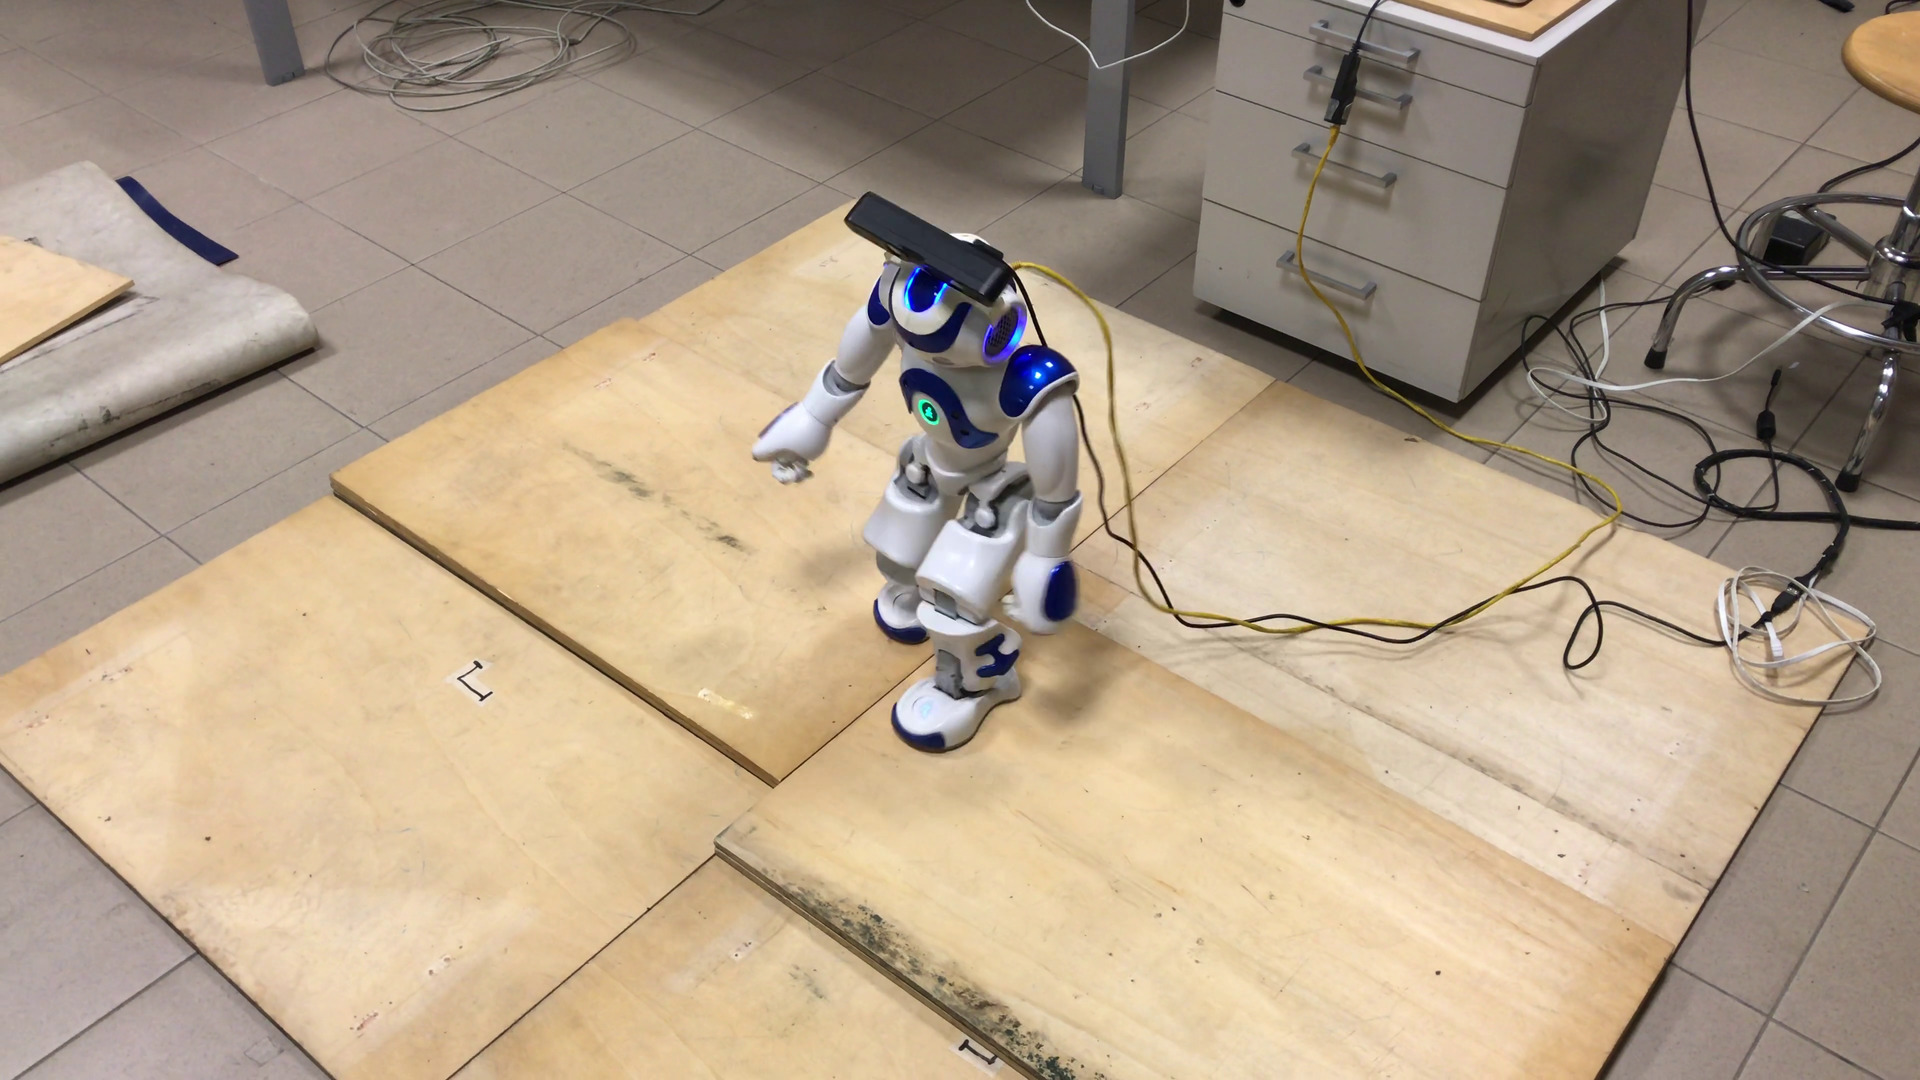
\includegraphics[width=\linewidth]
      {figures/experiments/unknown-env/video/07.png}
    \caption{Seventh step}
  \end{subfigure}\hspace*{\fill}
  \begin{subfigure}{0.48\textwidth}
    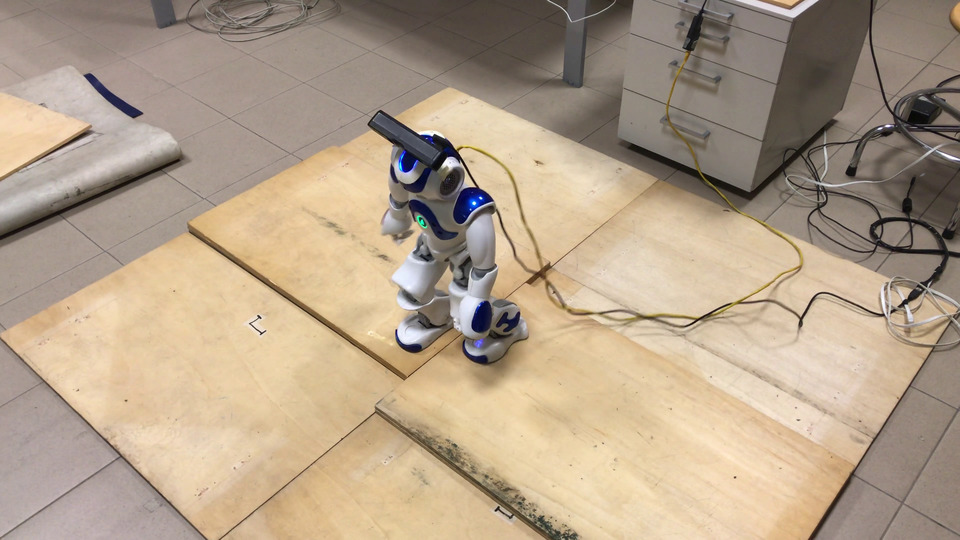
\includegraphics[width=\linewidth]
      {figures/experiments/unknown-env/video/08.png}
    \caption{Eighth step}
  \end{subfigure} \caption{The figures show the motion of the robot
      for the scenario ``Stair Climbing (Unknown Environment)''.
      The robot starts at 20 cm 
      from the first staircase (Fig. \ref{fig:exp:unkenv:frame1}). Before 
      starting the motion (Fig. \ref{fig:exp:unkenv:frame2}), an
      elevation map is built by the \texttt{elevation\_mapping} framework
      (Chapter \ref{ch:elevation-map-generation}),
      which receives the depth frames from the ASUS Xtion Pro placed 
      on top of the robot. The elevation map is sent to the planner, which 
      generates a footstep plan (Chapter \ref{ch:rrt-based-footstep-planning}).
      The footstep plan is then sent to the 
      robot, which executes the motion by using the Variable Height CoM
      IS-MPC (Chapter \ref{ch:vh-com-is-mpc}). The robot correctly manages to 
      climb the stairs without colliding with the staircases. Each staircase 
      has a height of 2 cm.}
  \label{fig:experiments:unkenv:videoframes}
\end{figure}

\begin{figure}
    \centering
    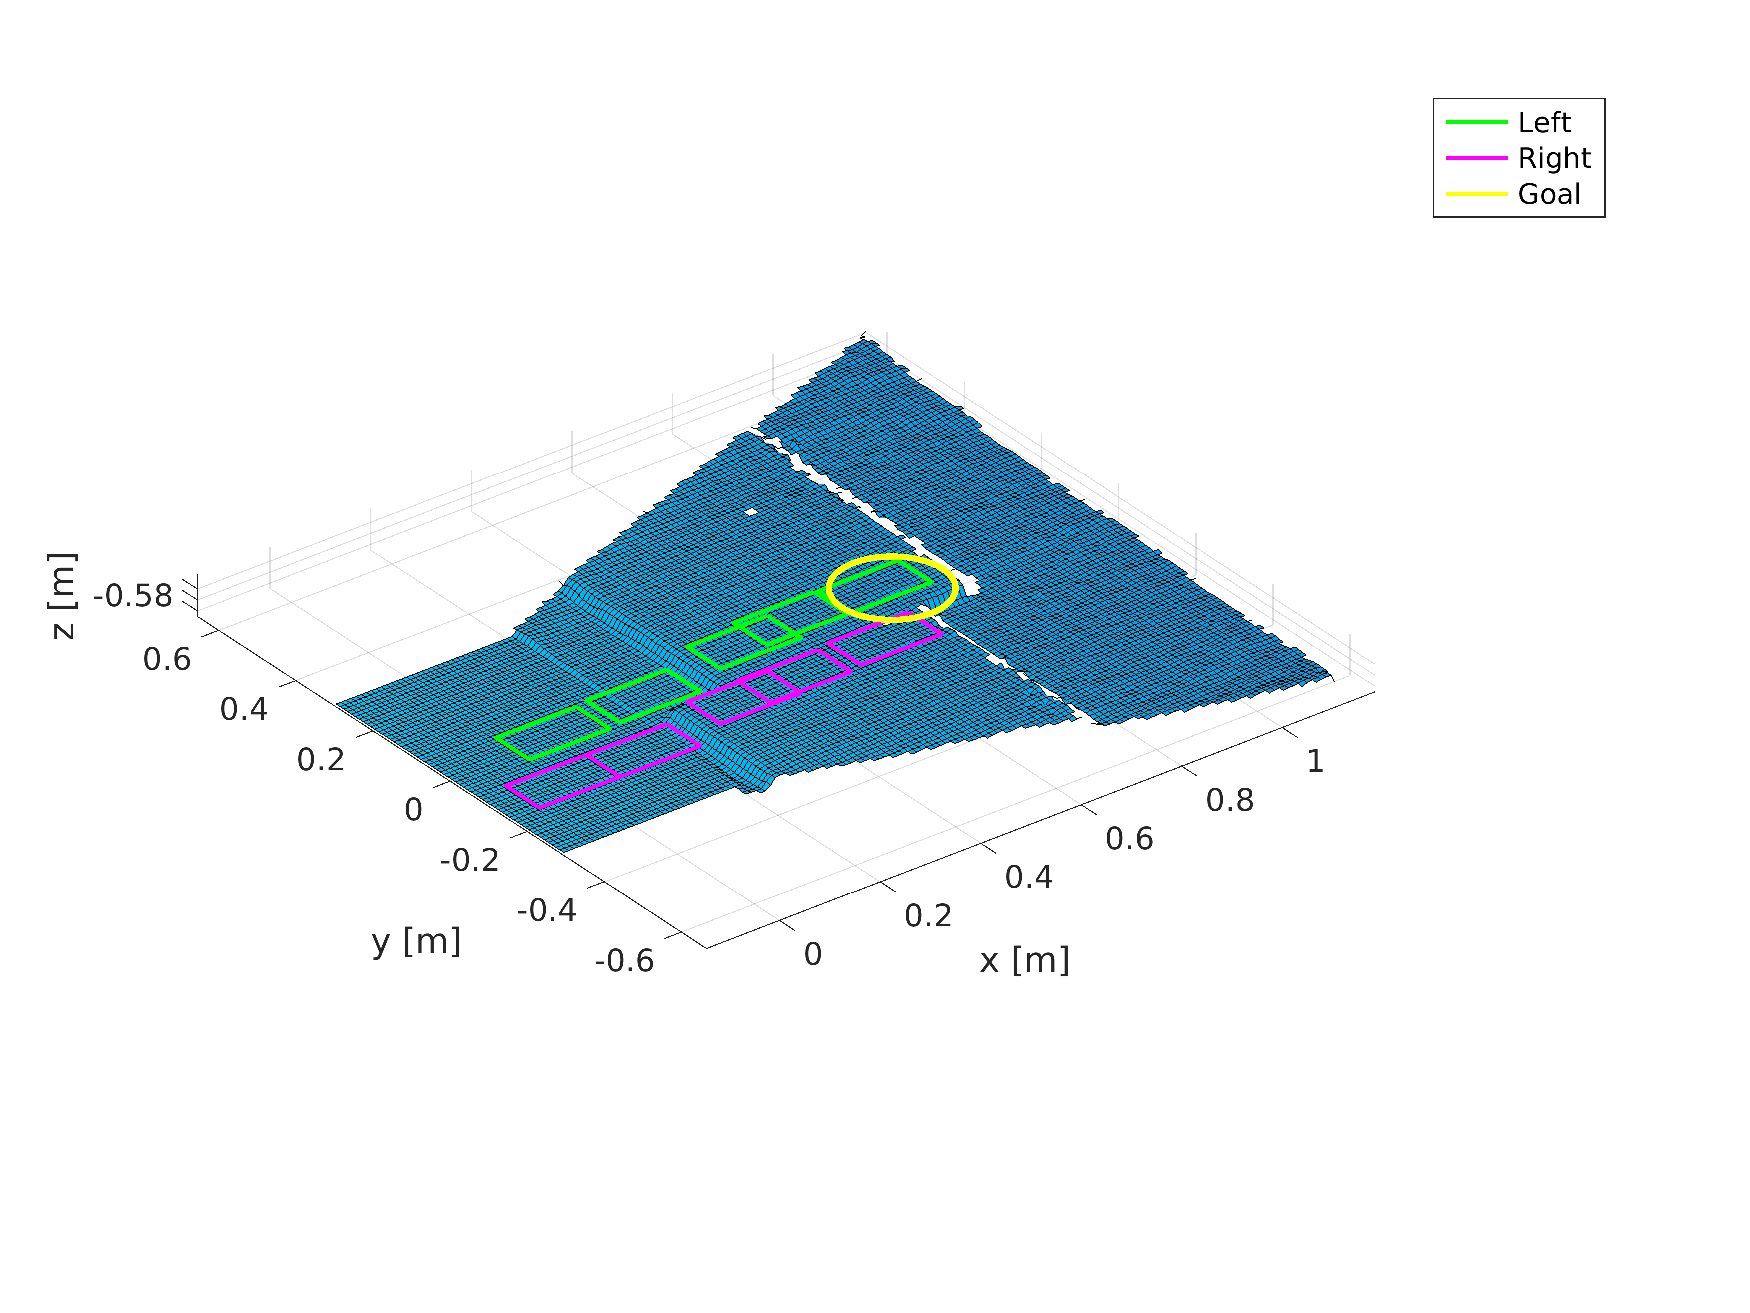
\includegraphics[width=0.95\textwidth]
        {figures/experiments/unknown-env/footstep-plan.pdf}
    \caption{Footstep plan generated for the scenario ``Stair Climbing in 
        Unknown Environments''.}
    \label{fig:experiments:unknown-env:footstep-plan}
\end{figure}
\begin{figure}
    \centering
    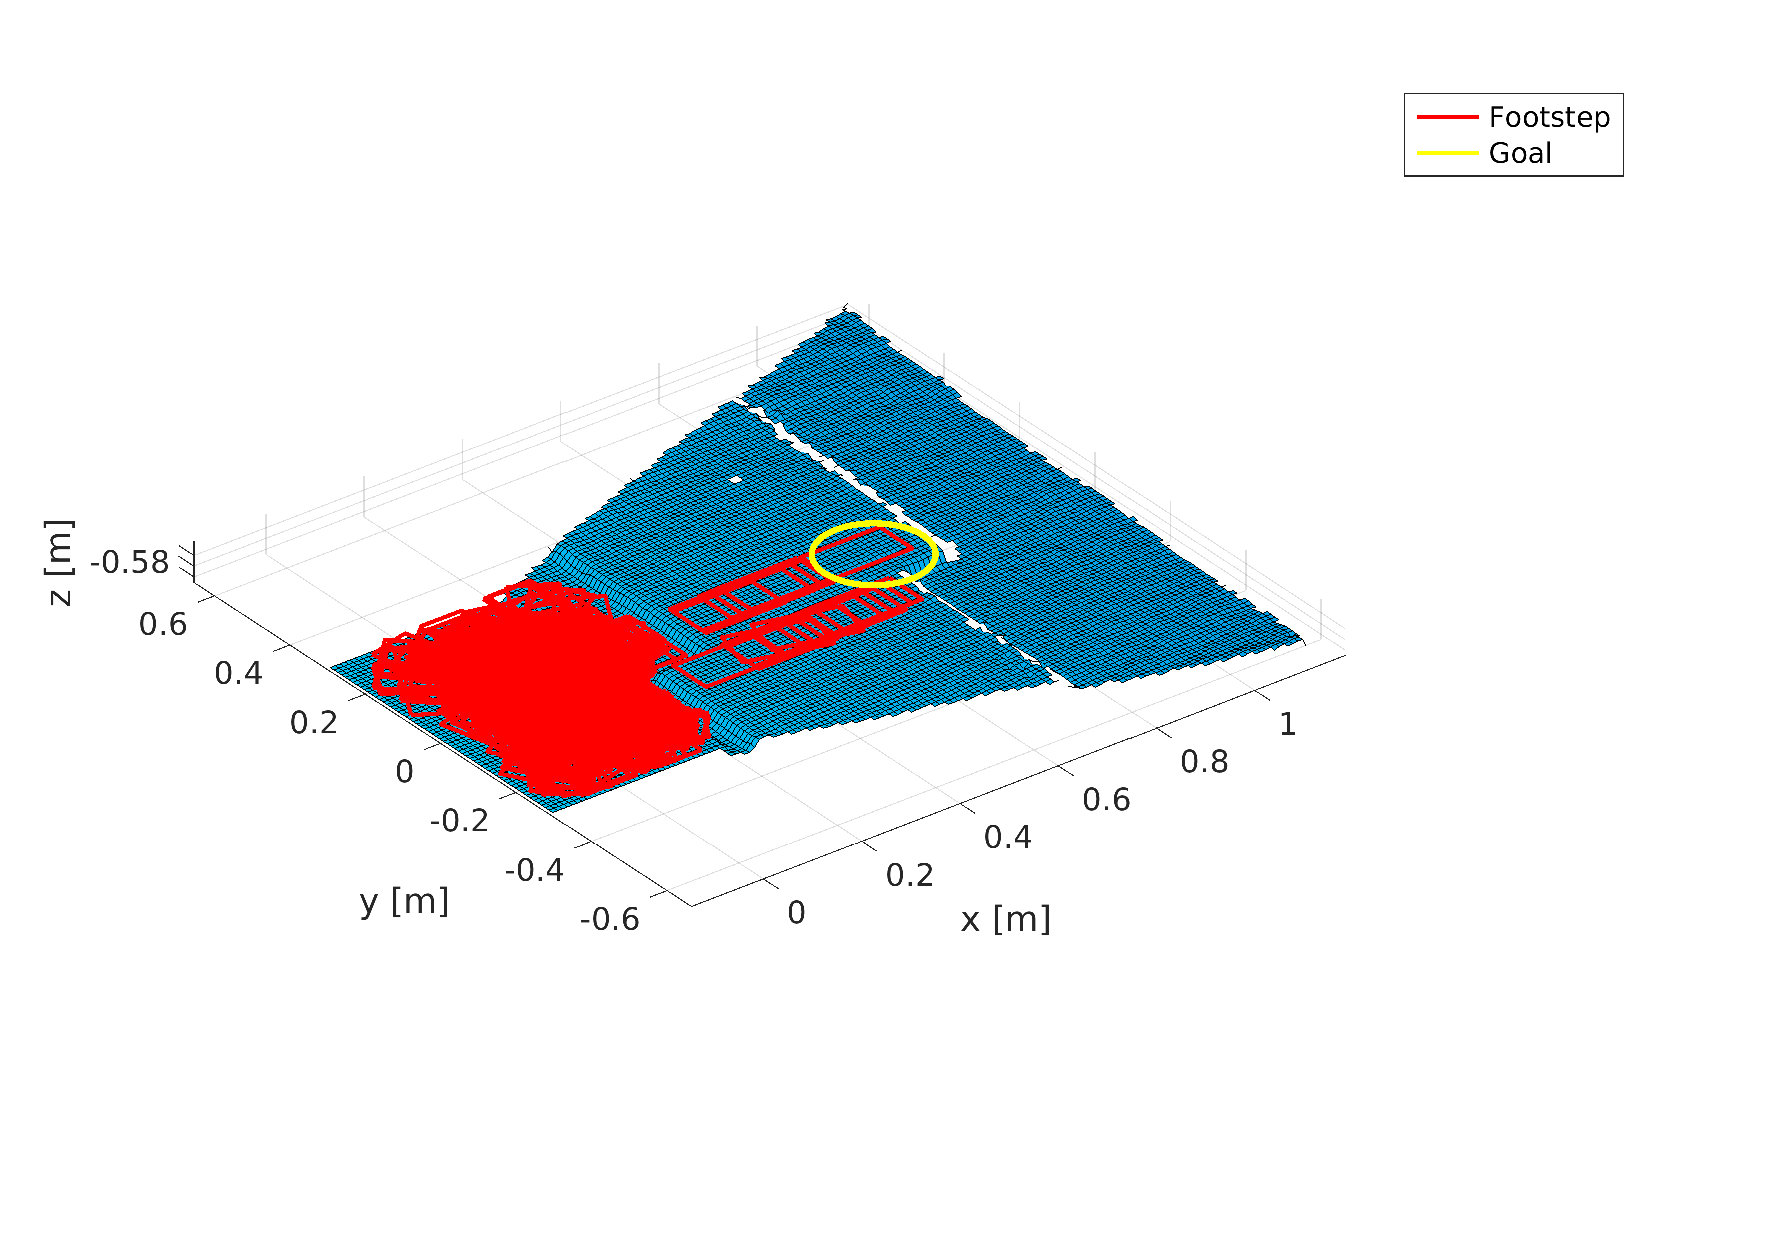
\includegraphics[width=0.95\textwidth]
        {figures/experiments/unknown-env/rrt-tree.pdf}
    \caption{Tree generated for the scenario ``Stair Climbing in 
        Unknown Environments''.}
    \label{fig:experiments:unknown-env:rrt-tree}
\end{figure}

